\documentclass[11pt]{article}
% packages
\usepackage[utf8]{inputenc}
\usepackage{geometry}
\usepackage[pdftex]{graphicx}
\usepackage{graphicx}
\usepackage{tabularx}
\usepackage{dsfont}
\usepackage{multirow}
\usepackage{amsmath,amsfonts,amssymb}
\usepackage{subcaption}
\usepackage{authblk}
\usepackage{placeins}
%hyperlinks options
\usepackage{hyperref}
\hypersetup{colorlinks=true,linkcolor=blue,filecolor=magenta,urlcolor=cyan,citecolor=cyan}
%bib options
\usepackage[backend=biber,style=authoryear,bibstyle=authoryear,natbib=true,
giveninits=true,uniquename=false,uniquelist=false,% firstinits=false,
maxcitenames=2,date=year, maxbibnames=99,url=false]{biblatex}
\geometry{left=20mm, top=20mm, right=20mm}
%float barrier
\usepackage{placeins}
 \addbibresource{Thèse.bib}
\title{Chapitre 3 : Analyse probabiliste des crues du Rhône à Beaucaire du XVI\textsuperscript{ème} siècle à aujourd'hui}
\author{Mathieu}


\begin{document}
\maketitle

\tableofcontents

\section{Introduction du chapitre}
	Quelques rappels d'intro aux méthodes d'analyse des crues histo:
	\cite{stedinger_flood_1986}\\
	Solutions quand le débit est connu\\
	Solution quand le débit n'est pas connu	\\
	Définition seuil et durée période histo\\
	%	plot positions (\citet{hirsch_techniques_1982}...)	\\
	Explication du concept de seuil de perception et de ses limites.\\
	durée de la période historique\\
	
	\paragraph{Méconnaissance du seuil}
	Le seuil de perception est un concept empirique qui ne prend une signification physique que dans certaines situations. Par exemple, imaginons une station hydrométrique dont la section n'a pas évolué au cours du temps et pour laquelle les débordements surviennent toujours au delà d'un même débit. Ces débordements (par exemple au-dessus d'une digue qui n'a subi aucune modification au cours du temps) laissent systématiquement une trace dans les écrits ou sur des infrastructures (marques de crue) suite aux dommages occasionnés. Cette situation parfaite existe rarement et le concept de seuil de perception peut être mis à mal par une variabilité temporelle de la perception des crues par les populations ripariennes. Néanmoins, l'utilisation du concept de seuil de perception est très souvent obligatoire pour exploiter les données de crues historiques. 
	
	\paragraph{Méconnaissance de la durée histo}Cette durée est pourtant importante dans le calcul de la binomiale. Il est erroné de considérer que la période historique démarre à la première crue et cela peut entrainer une sur-estimation de la fréquence d'occurrence. Plusieurs méthodes existent dans la littérature pour calculer cette durée et se basent sur (A COMPLETER...). 
		
\section{Méthodes d'analyse probabiliste d'un échantillon mixte de crues}
\label{sec:MethodoCh3}
	
	\subsection{Concepts de base et hypothèses}
	\label{subsec:conceptsdebase}
	
	\paragraph{} 
	
		L'utilisation d'occurrences de crues historiques pour l'analyse fréquentielle nécessite a minima l'hypothèse suivante : le débit de tous les événements de crue qui ont laissé une trace dans les archives ou les mémoires est supérieur à une certaine magnitude que l'on appellera "seuil de perception". Cela implique que pour toutes les années de la période historique sans mention de crue, on fait l'hypothèse que le débit inconnu a été inférieur au seuil de perception. Aussi, l'échantillon des crues supérieures au seuil de perception est supposé exhaustif. Il existe des méthodes d'analyse pour lesquelles il n'est pas nécessaire de connaitre précisément le débit des événements supérieurs au seuil de perception (voir notamment \citet{stedinger_flood_1986}). Le nombre de dépassements d'un seuil de perception pour une durée donnée est une information qui peut être exploitée en l'état. Ainsi, il faut considérer un échantillon mixte, composé d'une part de débits enregistrés en continu et d'autre part d'un nombre d'occurrences de crues supérieures à un seuil de perception. 
			
		\paragraph{}
		De manière similaire au Chapitre 1 (REF), on suppose que le débit maximum annuel des périodes continues et historiques $Q$ est une variable aléatoire $iid$ qui suit une distribution GEV, de paramètres $\boldsymbol{\theta} = (\mu,\sigma,\xi)$ (respectivement : position, échelle, forme). Pour simplifier, on suppose ici que le paramètre de forme $\xi$ est différent de zéro (loi de Gumbel). Ainsi, on a la fonction de répartition de la GEV : $F(x;\boldsymbol{\theta}) = e^{-(1-\xi(\frac{x - \mu}{\sigma}))^{1/\xi}}$. Lorsque le paramètre de forme est strictement positif ($\xi > 0$), on se trouve dans le cas "loi de Weibull" avec une borne supérieure et des quantiles supérieurs à ceux d'une loi de Gumbel. Dans le cas contraire ($\xi < 0$), il s'agit du cas "loi de Fréchet" de la distribution GEV. Les débits de l'échantillon de maximum annuels enregistrés en continu pendant $j$ années $\boldsymbol{q}= (q_t)_{t=1,...,j}$ sont ici supposés parfaitement connus et dans un premier temps non affectés d'une quelconque incertitude. L'échantillon historique est composé de $k$ événements ayant dépassé le seuil de perception $S$ sur une période de $n$ années. Le seuil de perception n'a donc pas été dépassé pour les $n-k$ années restantes. Ainsi, la probabilité de dépassement du seuil peut s'écrire :
		
		\begin{equation}
			\pi = \biggl( 1 - F(S;\boldsymbol{\theta})\biggl) = 1 - e^{-\biggl(1-\xi\bigl(\frac{S-\mu}{\sigma}\bigl)\biggl)^{1/\xi} }		
		\end{equation}
			 
	On suppose que $k$, le nombre de dépassements du seuil de perception, peut être estimé par une loi binomiale de paramètres $n$ et $\pi$, soit $\mathcal{B}(n,\pi)$. On peut alors écrire la fonction de vraisemblance (équation \ref{eq:Gev_Binom}) qui est fonction d'un échantillon mixte de données composé des débits maximum annuels de la période continue $(q_t)_{t=1,...,j}$ et du nombre de dépassements du seuil de perception $k$ durant la période historique $n$ :
		
			\begin{equation}
			L(\boldsymbol{\theta} ; \boldsymbol{q}, k) = \underbrace{\prod_{t=1}^j f\left(q_t;\boldsymbol{\theta}\right)}_{\mathrm{a}} \underbrace{\left\{\left(\begin{array}{l}
			n \\
			k
			\end{array}\right) F\left(S;\boldsymbol{\theta}\right)^{n-k}\left[1-F\left(S;\boldsymbol{\theta}\right)\right]^k\right\}}_{\mathrm{b}} \\
			\label{eq:Gev_Binom}
			\end{equation}
			
			Ici, le terme $\mathrm{a}$ représente la vraisemblance pour les données continues et le terme $\mathrm{b}$ la vraisemblance pour les données historiques. L'application de la formule de Bayes permet de calculer la distribution a posteriori des paramètres $\boldsymbol{\theta}$ sachant les données :
			
			\begin{equation}
				p(\boldsymbol{\theta} \mid \boldsymbol{q},k) \propto L(\boldsymbol{\theta};\,\boldsymbol{q},k) p(\boldsymbol{\theta})
				\label{eq:BayesBinom}
			\end{equation}
	
		Le terme $P(\boldsymbol{\theta})$ représente ici la distribution a priori des paramètres qu'il faudra éliciter. La distribution a posteriori est explorée via une méthode bayésienne MCMC (notamment décrite par \citet{coles_classical_2001}). Cette distribution a posteriori représente l'incertitude d'échantillonnage du modèle par $r$ jeux de paramètres : $\boldsymbol{\Theta} = (\boldsymbol{\theta_1},...,\boldsymbol{\theta_r})$. Le jeu de paramètres qui maximise la distribution a posteriori est appelé maxpost et s'écrit $\boldsymbol{ \hat{\theta} }$. Pour l'ensemble des simulations du présent chapitre, les a priori des paramètres de la distribution GEV seront les suivants : distribution plate (uniforme et très peu informative) pour $mu$ et $sigma$, et distribution gaussienne de moyenne zéro et d'écart type 0.2 pour $xi$. Cet a priori peu informatif du paramètre de forme est notamment cohérent avec les suggestions de \citet{martins_generalized_2000}.
	
	
%	\paragraph{Description difficultés de détermination du seuil et durée historique}
%	Complexité de déterminer le seuil\\
%	Complexité de déterminer la durée de la période historique \citep{prosdocimi_german_2018}). 			Attention aux confusions entre date de début de la période et durée de la période. \\

	
	\subsection{Propagation de l'incertitude hydrométrique des mesures systématiques (modèle A)}
	\label{subsec:modA}
	
	\paragraph{}
	Dans la section précédente, l'incertitude des débits maximum annuels de la période continue est supposée négligeable. Cette incertitude pouvant atteindre 30 \% à Beaucaire (REF Chap 1), il semble pragmatique de la considérer. Comme décrit dans la section REF du Chapitre 1, cette incertitude hydrométrique est représentée par $s = 500$ réalisations : $(q_t^{(i)})_{t=1,...,j;\,i=1,...,s}$. Elle peut être propagée aux estimations des paramètres de l'équation \ref{eq:Gev_Binom} en estimant un jeu de paramètres pour chacune des $s$ réalisations, soit $(\boldsymbol{\theta}
	^{(i)})_{i=1,...,s}$. Au total, $r \times s$ jeux de paramètres sont estimés et représentent l'effet combiné de l'incertitude d'échantillonnage et de l'incertitude hydrométrique des données continues, on a donc $(\boldsymbol{\theta}^{(i)}_p)_{p=1,...,r;\, i=1,...,s}$. Le jeu de paramètres le plus probable est calculé en utilisant l'échantillon maxpost de débits maximum annuels (CHAPITRE 1) sur lequel on estime le jeu de paramètres maxpost de l'équation \ref{eq:Gev_Binom}. Le modèle décrit ci-dessus sera appelé "modèle A". La propagation des incertitudes hydrométriques de la période continue telle que décrite ici sera effectuée similairement pour les trois modèles définis dans les sections suivantes.
	
	\subsection{Seuil de perception incertain (modèle B)}
	\label{subsec:modB}
	
		\paragraph{}
		Afin de considérer dans le modèle fréquentiel une prise en compte pragmatique de la méconnaissance du seuil de perception, il est possible de considérer ce seuil comme étant un paramètre à part entière du modèle. Il ne s'agit pas ici de considérer un seuil de perception variable au cours du temps, quoi que de nombreux exemples dans la littérature font l'hypothèse de plusieurs seuils de perception successifs dont le débit est différent. Un seul seuil de perception est ici considéré pour l'ensemble de l'échantillon, mais sa valeur est incertaine et est déterminée par le modèle. L'impact de la méconnaissance du seuil est ainsi répercuté sur l'incertitude des résultats. Dans la section précédente, le seuil de perception faisait déjà partie du modèle (équation \ref{eq:Gev_Binom}), mais sa valeur était supposée connue, ce qui n'est ici plus le cas. La vraisemblance s'écrit alors : 
		
				\begin{equation}
				L(\boldsymbol{\theta}, S ; \boldsymbol{q}, k) =\prod_{t=1}^j f\left(q_t;\boldsymbol{\theta}\right) \left\{\left(\begin{array}{l}
				n \\
				k
				\end{array}\right) F\left(S;\boldsymbol{\theta}\right)^{n-k}\left[1-F\left(S;\boldsymbol{\theta}\right)\right]^k\right\} \\
				\label{eq:Gev_Binom_uS}
				\end{equation}
				
		On peut alors écrire une nouvelle distribution a posteriori : 			
				
				\begin{equation}
					p(\boldsymbol{\theta}, S \mid \boldsymbol{q},k) \propto L(\boldsymbol{\theta},S;\,\boldsymbol{q},k) p(\boldsymbol{\theta},S)
					\label{eq:Bayes_uS}
				\end{equation}
			
		La distribution des paramètres a posteriori de ce modèle reflètent l'incertitude hydrométrique de la période continue, l'incertitude d'échantillonnage, ainsi que l'incertitude du seuil de perception. Ce modèle sera nommé "modèle B" dans les sections suivantes.
		

	\subsection{Durée de la période historique incertaine (modèle C)}
	\label{subsec:modC}
	
		\paragraph{}
		L'équation \ref{eq:Gev_Binom} repose à la fois sur le fait que le seuil de perception $S$ et la durée de la période historique $n$ sont connus. De la même manière que décrit à la section précédente pour le seuil, la durée (et donc l'année qui marque le début) de la période historique peut être complexe à déterminer. Généralement, la date qui marque la fin de la période historique est parfaitement connue, car elle correspond également au début des enregistrements continus. En revanche, la date du début de l'échantillon historique (que l'on appellera $t*$), à partir de laquelle toutes les crues supérieures au seuil de perception seront connues, correspond à une période lointaine et relativement mal connue d'un l'échantillon historique. Ainsi, nous proposons ici de considérer la durée de la période historique $n$ comme étant un paramètre à part entière du modèle fréquentiel. Le seuil de perception est en revanche supposé parfaitement connu dans ce cas de figure. La vraisemblance s'écrit alors : 
		 
				\begin{equation}
				L(\boldsymbol{\theta}, n ; \boldsymbol{q}, k) = \prod_{t=1}^j f\left(q_t;\boldsymbol{\theta}\right) \left\{\left(\begin{array}{l}
				n \\
				k
				\end{array}\right) F\left(S;\boldsymbol{\theta}\right)^{n-k}\left[1-F\left(S;\boldsymbol{\theta}\right)\right]^k\right\} \\
				\label{eq:Gev_Binom_uN}
				\end{equation}
				
		On peut alors exprimer une nouvelle distribution a posteriori :
		
				\begin{equation}
					p(\boldsymbol{\theta}, n \mid \boldsymbol{q},k) \propto L(\boldsymbol{\theta},n;\,\boldsymbol{q},k) p(\boldsymbol{\theta},n)
					\label{eq:Bayes_uN}
				\end{equation}
			
		La méconnaissance de la durée de la période historique $n$ est donc prise en compte dans le modèle et est a un impact sur l'incertitude des résultats. Ce modèle sera nommé "modèle C" dans les sections suivantes. 
	
	\subsection{Seuil de perception et durée de la période historique incertains (modèle D)}
	\label{subsec:modD}	
	
	\paragraph{}
	Le seuil de perception $S$ et la durée de la période historique $n$ étant par définition reliés (un seuil de perception étant valide sur une durée donnée) on peut construire un modèle qui représente en même temps la méconnaissance autour de ces deux paramètres. La vraisemblance de ce modèle s'écrit :  
	
					\begin{equation}
			L(\boldsymbol{\theta}, S, n ; \boldsymbol{q}, k) = \prod_{t=1}^j f\left(q_t;\boldsymbol{\theta}\right) \left\{\left(\begin{array}{l}
			n \\
			k
			\end{array}\right) F\left(S;\boldsymbol{\theta}\right)^{n-k}\left[1-F\left(S;\boldsymbol{\theta}\right)\right]^k\right\} \\
			\label{eq:Gev_Binom_SN}
			\end{equation}
		
		On peut exprimer la vraisemblance du modèle telle que :
					
			\begin{equation}
				p(\boldsymbol{\theta}, S, n \mid \boldsymbol{q},k) \propto L(\boldsymbol{\theta},S, n;\,\boldsymbol{q},k) p(\boldsymbol{\theta},S, n)
				\label{eq:Bayes_uSN}
			\end{equation}

	Ce modèle pour lequel $S$ et $n$ sont incertains sera nommé "modèle D" dans les sections suivantes. 
	
	\subsection{Débit des crues historiques compris dans un intervalle (modèle E)}
	\label{subsec:modE}	
		
	\paragraph{} Dans certains cas, le débit des crues historiques supérieures au seuil de perception est connu. De façon similaire au modèle binomial décrit précédemment, on peut faire l'hypothèse que le débit maximum annuel de toutes les années de la période historique sans mention de crues est inférieur au seuil de perception. Le débit des crues connues peut ensuite être pris en compte dans le modèle fréquentiel décrit par \citet{stedinger_flood_1986}. Il est également possible de considérer que le débit des crues historiques n'est pas parfaitement connu, mais qu'il est compris dans un intervalle de confiance. Plusieurs exemples d'un tel modèle existent dans la littérature (par exemple : \cite{payrastre_usefulness_2011} ou Parkes REF). La vraisemblance d'un tel modèle peut s'écrire : 

		\begin{equation}
					L(\boldsymbol{\theta} ; \boldsymbol{q}, \boldsymbol{y}) =\prod_{t=1}^j f\left(q_t;\boldsymbol{\theta}\right) \prod_{i=1}^k \left[F(y_{i}^{sup},\boldsymbol{\theta} ) - F(y_i^{inf},\boldsymbol{\theta})\right]
		\label{eq:Censure}
		\end{equation}
					
		\paragraph{}où $q_t$ correspond aux $j$ crues de la période continue et $y_i$ aux $k$ crues de la période historique dont le débit est compris dans l'intervalle d'incertitude à 95\% $\left[y_i^{inf} ; y_i^{sup}\right]$. La distribution a posteriori du modèle s'écrit alors : 
				
		\begin{equation}
			p(\boldsymbol{\theta} \mid \boldsymbol{q},\boldsymbol{y}) \propto L(\boldsymbol{\theta};\,\boldsymbol{q},\boldsymbol{y})p(\boldsymbol{\theta})
		\label{eq:Bayes_Censure}
		\end{equation}

	\paragraph{} Ce modèle sera nommé "modèle E" dans les sections suivantes. Ici aussi, l'incertitude des débits de la période continue est propagée tel que décrit dans la section REF. On pourra comparer les quantiles obtenus avec le modèle E pour lequel le débit des crues historiques est connu (dans un intervalle), avec les résultats des modèles binomiaux pour lesquels seul le nombre de dépassements $k$ du seuil de perception est connu.
	

	\subsection{Distribution empirique d'un échantillon mixte}
	\label{subsec:DistEmpirique}
	
		\paragraph{} Le classement en fréquence des crues dans le cas d'un échantillon mixte peut poser problème, notamment quand le débit des crues historiques n'est pas connu, n'ayant d'autre information que le dépassement d'un seuil de perception. \citet{hirsch_probability_1987} propose une méthode pour le classement en fréquence d'un échantillon mixte quand le débit des crues est connu. Pour un échantillon continu de crues classé par valeurs décroissantes : $q(1) \geq ... \geq q(j)$, la fréquence empirique au dépassement s'écrit : $f_i = P(\boldsymbol{Q} > q(i)) = \frac{i-\alpha}{j+1-2\alpha}$. Nous prenons ici $\alpha = 0.5$ (REF HAZEN). Pour un échantillon mixte composé d'un échantillon continu de $j$ débits maximum annuels et de $k$ crues historiques supérieures à un seuil $S$ couvrant $n$ années, il faut raisonner sous la forme de deux sous-échantillons. Le nombre de crues supérieures au seuil $S$ sur la période complète est ici noté $NS$, et la durée de la période complète correspond à $j + n$ années. On a d'après \citet{hirsch_probability_1987} :
		
		\begin{equation}	
		P(\boldsymbol{Q} > q(i)) = \begin{cases}\dfrac{i-\alpha}{NS+1-2 \alpha} \dfrac{NS}{j+n}, & i=1, \ldots, NS \\ \dfrac{NS}{j+n}+\dfrac{j+n-NS}{j+n} \dfrac{(i-NS-\alpha)}{(j-NS+1-2\alpha)}, & i=NS+1, \ldots, j+k\end{cases}
		\label{eq:FreqHisto}	
		\end{equation}
%	
%		\begin{equation}	
%		P(\boldsymbol{Q} > q(i)) = \begin{cases}\frac{i-\alpha}{NS+1-2 \alpha} \frac{NS}{j+n}, & i=1, \ldots, NS \\ \frac{NS}{j+n}+\frac{j+n-NS}{j+n} \frac{(i-NS-\alpha)}{(j-NS+1-2\alpha)}, & i=NS+1, \ldots, j+k\end{cases}
%		\label{eq:FreqHisto}	
%		\end{equation}
%		
	
	\paragraph{} Lorsque le débit des crues historiques est connu, on peut classer l'ensemble des crues supérieures au seuil (de la période continue et historique) par ordre décroissant en leur attribuant le rang $i$. Lorsque le débit des crues historiques n'est pas connu, il n'est pas possible de classer cet échantillon. Une manière de contourner ce problème est de tirer aléatoirement le rang $i$ de l'ensemble des crues supérieures au seuil. Ce classement est aléatoire, mais il permet d'affecter une fréquence empirique aux crues. Ainsi, on peut comparer la fréquence empirique des observations de crues aux ajustements statistiques décrits dans les sections précédentes afin de vérifier leur cohérence. 
		
		
\section{Données disponibles}

	\subsection{Échantillon mixte de crues du Rhône à Beaucaire}
	\paragraph{} L'échantillon de crues du Rhône à Beaucaire est constitué de deux types de données : premièrement, un échantillon continu de débits maximum annuels mesurés de 1816 à 2020. Ces débits ont été estimés au chapitre 1 (REF) et leur incertitude hydrométrique est représentée par 500 réalisations de l'échantillon. Deuxièmement, une collection de témoignages de crues historiques de 1500 à 1816, tirés de la base HISTRHÔNE et classées en deux catégories tel que décrit au chapitre 2 (REF). Les seuils de perception correspondant aux deux échantillons ne sont pas précisément connus, mais on suppose que le seuil $S3$ qui correspond aux crues des catégories C3 et C4 se situe aux alentours de 7000 $m^3/s$, et le seuil $S4$ qui correspond aux crues de la catégorie C4 uniquement se situe aux alentours de 9000 $m^3/s$ (VALEURS DEFINIES AU CHAP 2). La figure \ref{fig:EchMixte} présente l'ensemble des données disponibles. 
	
	\begin{figure}[h]
		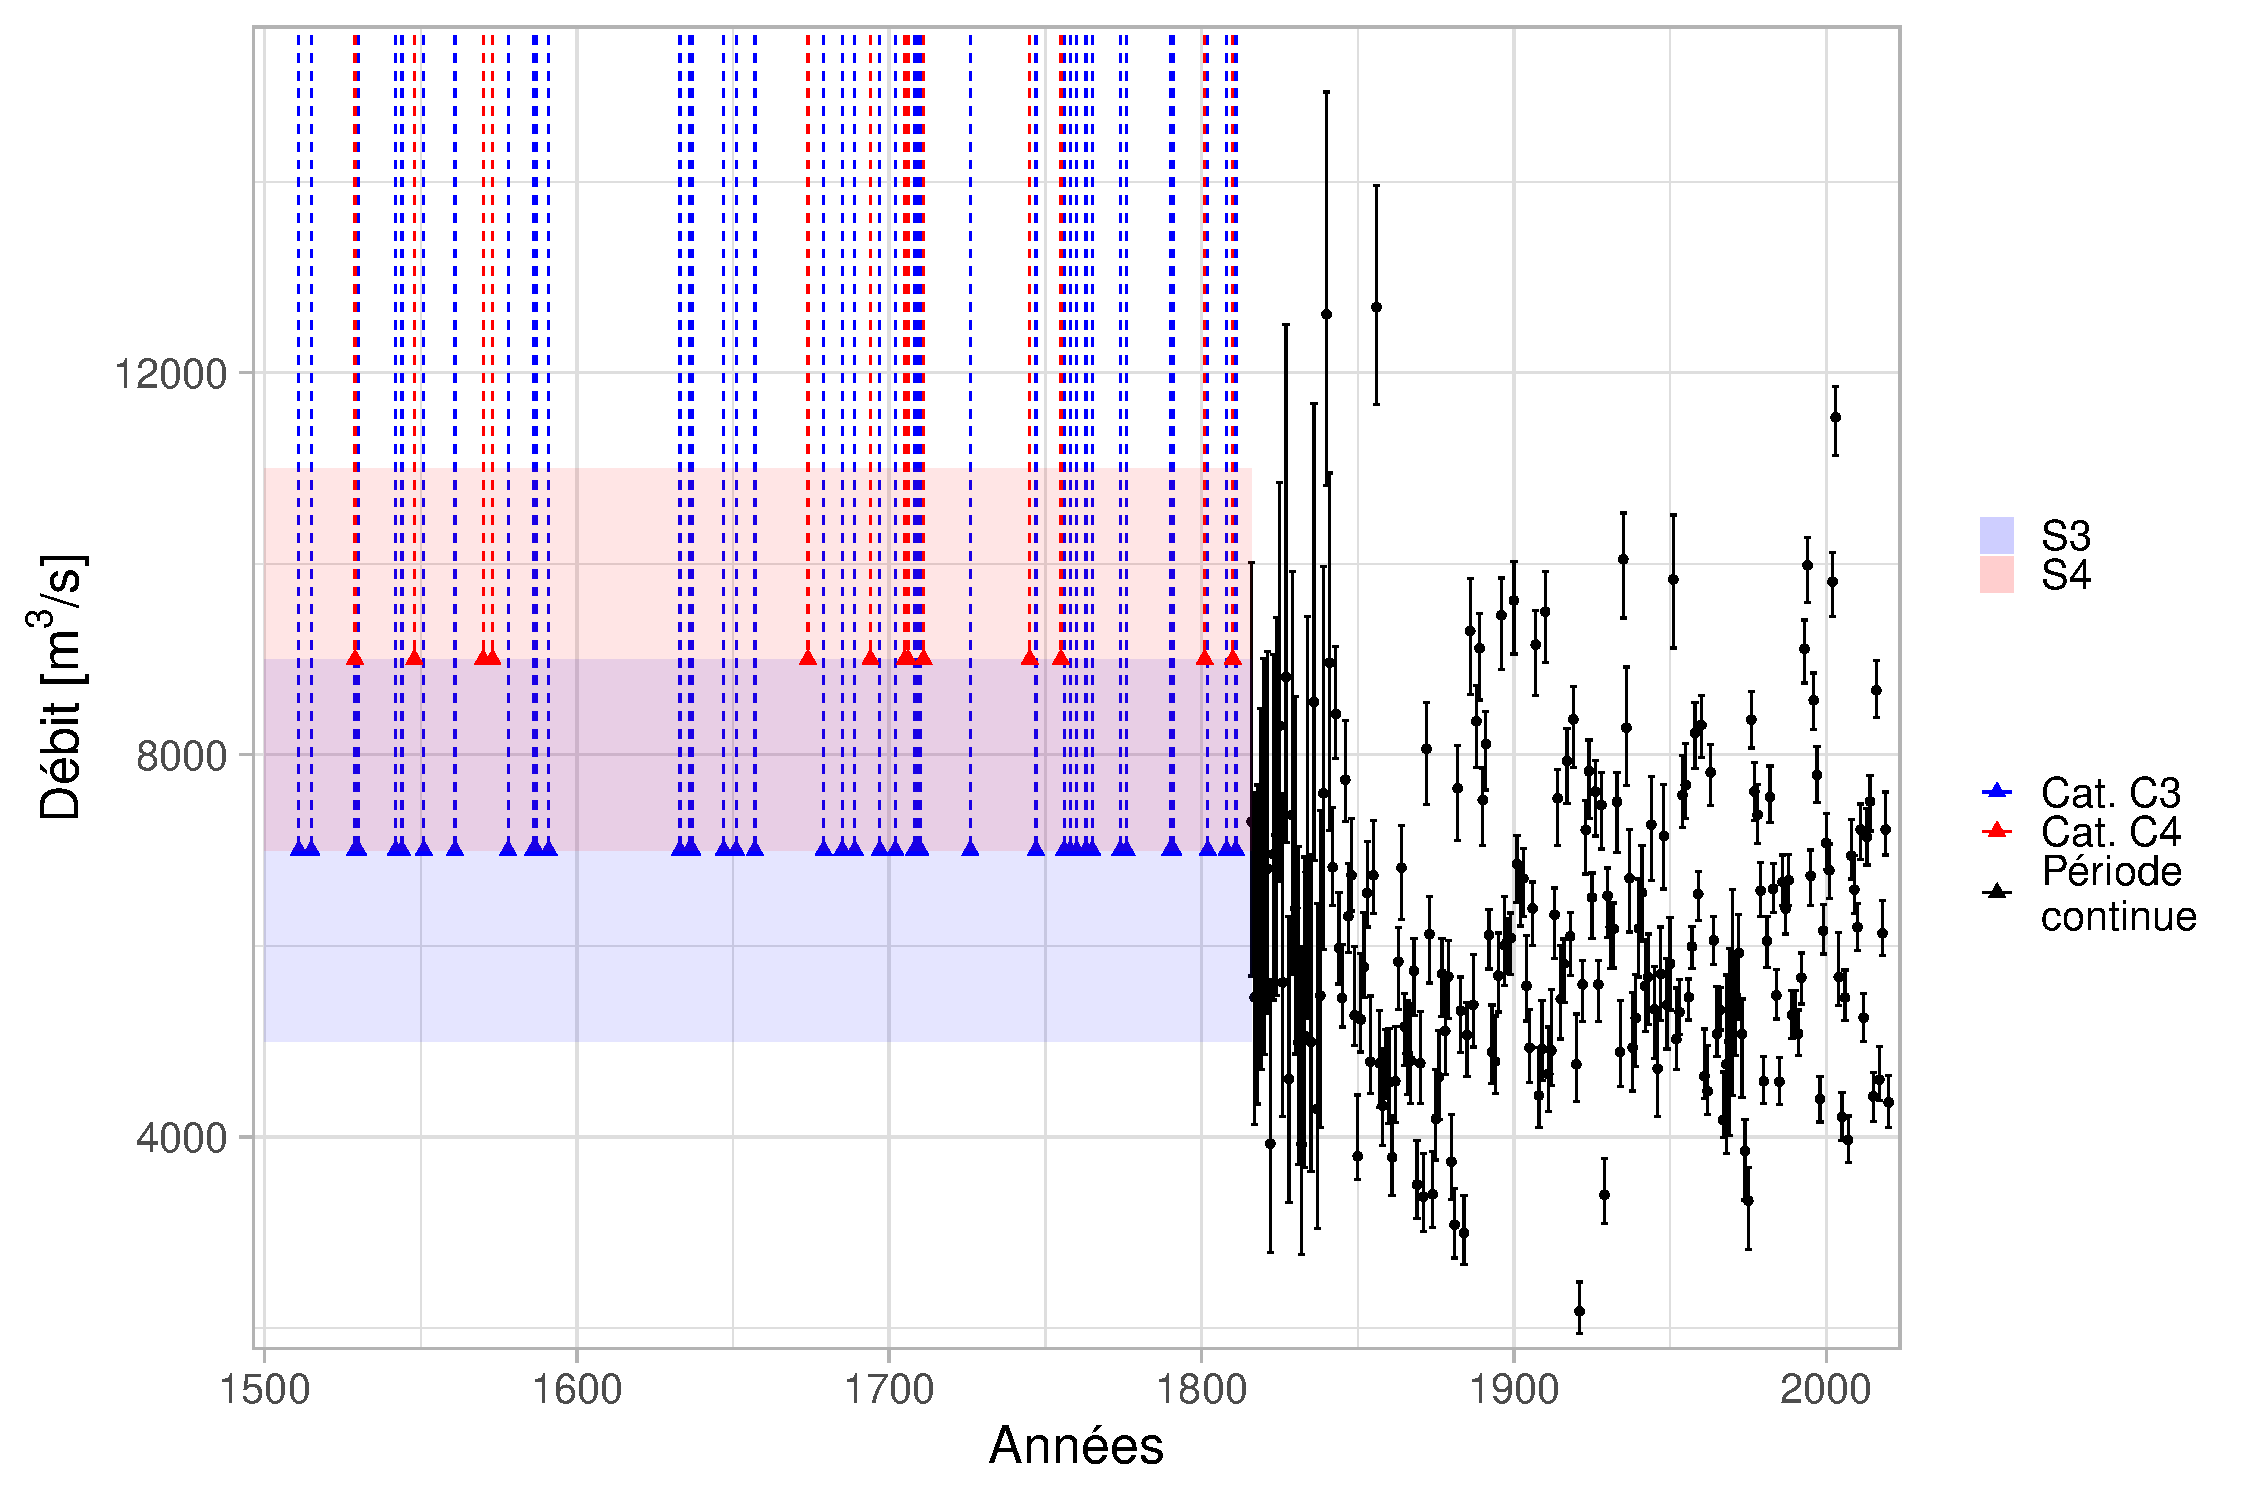
\includegraphics[width=.9\linewidth]{Figures/EchMixteBcr.pdf}	
		\caption{Échantillon de crues du Rhône à Beaucaire. L'incertitude à 95\% autour des seuils de perception est représentée par les bandeaux bleu et rouge ("S3" et "S4)}
		\label{fig:EchMixte}
	\end{figure}
	

	\subsection{Homogénéité des données}
	\label{subsec:homog}
	\paragraph{} L'homogénéité des données est un pré-requis essentiel à l'analyse fréquentielle des crues en contexte stationnaire, car cette dernière repose sur l'hypothèse que les variables étudiées sont dites $iid$ (indépendantes et identiquement distribuées). C'est-à-dire que les processus statistiques pouvant être utilisés pour modéliser la distribution des crues ne changent pas dans le temps. Ainsi, pour une station donnée, une même distribution peut être utilisée pour modéliser les crues du XVI\textsuperscript{ème} et du XXI\textsuperscript{ème} siècle. Étant donné que deux types d'échantillons sont ici utilisés, deux types de tests statistiques sont appliqués dans les sections suivantes pour étudier l'homogénéité de ces données. 

	\subsubsection{Données continues}
	
	\paragraph{} Trois tests seront utilisés pour qualifier l'homogénéité de l'échantillon de données continues : Le test de Pettitt (REF) et la procédure de segmentation développée par \citet{darienzo_detection_2021-1} qui permettent de détecter des ruptures dans les séries temporelles, ainsi que le test de Mann-Kendall (REF) qui permet de détecter l'existence de tendances. Les ruptures sont des changements soudains (i.e. les données ont une distribution différente avant et après un instant $t$, par exemple suite à un changement d'instrumentation), tandis que les tendances représentent des changements progressifs dans la distribution des données au cours du temps (par exemple : un changement des conditions ). Parmi ces trois tests, seule la procédure de segmentation de \citet{darienzo_detection_2021-1} permet de considérer l'incertitude des données d'entrée (déterminée au Chapitre 1 (REF)).
	
	\paragraph{} La p-value des tests de Pettitt et Mann-Kendall appliqués à la série maxpost des débits maximum annuels à Beaucaire est respectivement de 0.15 et 0.41. Au risque d'erreur 5\%, on peut conclure qu'il n'existe pas de tendance ou de rupture dans la série. Il faut cependant s'assurer que ce résultat est toujours vrai lorsque l'on considère les incertitudes de la série.
			
	\paragraph{} L'application de la procédure de segmentation de \citet{darienzo_detection_2021-1} à la série de débits maximum annuels avec incertitude a conclu que le nombre optimal de segments pour la chronique de Beaucaire était de 1, et ce quel que soit le critère de segmentation considéré (AIC, BIC, HQC ou DIC). On peut ainsi conclure qu'aucune rupture n'existe dans les données. L'échantillon de données continues peut être considéré homogène suite aux tests statistiques réalisés. 
	
%	\paragraph{} Afin de d'étudier l'existence de tendances dans la série en considérant les incertitudes, le test de Mann-Kendall a été appliqué aux 500 réalisations possibles. Seulement 20\% des 500 p-values calculées sont inférieures à 0.05. Au risque d'erreur 5\%, on peut alors conclure que seulement 20\% des 500 réalisations de la série comportent une tendance. On peut calculer une valeur théorique ... A quelle valeur faudrait-il s'attendre pour considérer que c'est homogène (Benjamin ?) 

		
	\subsubsection{Données historiques}
	
	\paragraph{} Les données pré-enregistrements continus (ou historiques) utilisées ici prennent la forme d'occurrences de crues supposées supérieures à un seuil de perception. Comme décrit par \citet{lang_towards_1999}, la fréquence des occurrences de crues supérieures à un seuil est supposée suivre un processus de Poisson. Afin de vérifier l'homogénéité des occurrences de crues, il est possible de calculer un intervalle de confiance autour du nombre cumulé de crues découlant du processus de Poisson. Si les occurrences de crues cumulées "sortent" de cet intervalle de confiance, alors leur fréquence d'occurrence est supposée non-stationnaire. 
	
	\paragraph{} Ces intervalles de confiance ont été calculés pour l'échantillon de crues pré-enregistrements continus du Rhône à Beaucaire. La période historique est supposée débuter en 1500 et se termine à l'année des premiers enregistrements continus de hauteur d'eau, en 1816. Les deux échantillons testés ici reflètent deux seuils de perception, $S3$ et $S4$, et on a $S3 < S4$. 

	\begin{figure}[h]
		\centering
		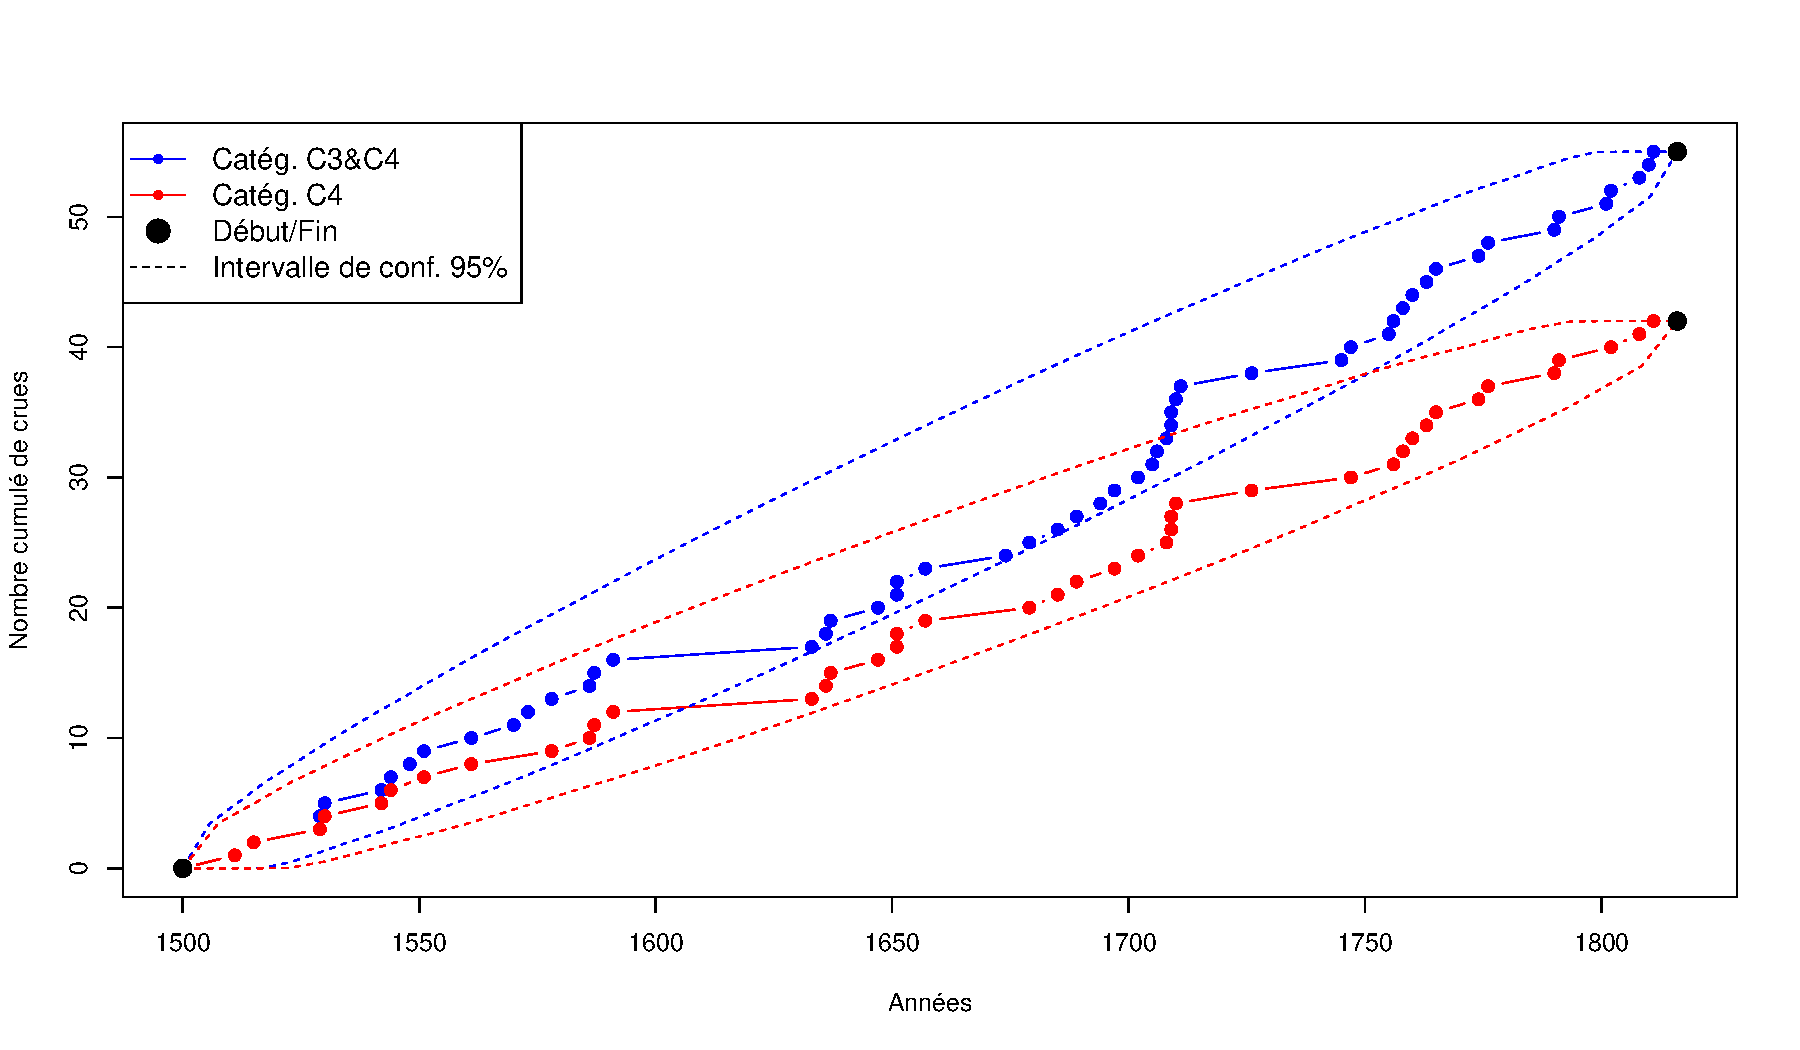
\includegraphics[width=.8\linewidth]{Figures/Poisson_C3-C4_FR.pdf}	
		\caption{Nombre de crues cumulé et intervalles de confiance à 95\% du processus de 						Poisson, pour deux échantillons d'occurrences de crues supérieures aux seuils $S3$ ou $S4$ à Beaucaire 							(1500-1816)}
		\label{fig:Poisson_C3-C4}
	\end{figure}		
	
	\paragraph{} Sur la figure \ref{fig:Poisson_C3-C4}, on remarque que les nombre cumulés de crues des deux échantillons sont compris dans les intervalles de confiance à 95\% des processus de Poisson, ils peuvent donc être tous deux considérés homogènes. L'échantillon correspondant au seuil $S3$ (en bleu) se rapproche de la borne inférieure de l'intervalle de confiance au XVII\textsuperscript{ème} siècle, mais revient rapidement dans des valeurs moyennes à la faveur de nombreuses crues supérieures au seuil au début du XVIII\textsuperscript{ème} siècle. 
	
	\paragraph{} L'échantillon continu de débits maximum annuels (1816-2020) sera par la suite artificiellement "dégradé" pour reproduire des durées de chroniques plus usuelles. Ainsi, les crues dont le débit maxpost est supérieur au seuil considéré sont retenues dans l'échantillon. Cette période "dégradée" commence au début de la chronique, en 1816, et se termine en 1970, à la mise en fonctionnement de la station de Beaucaire Restitution. Deux seuils de perception similaires aux seuils $S3$ et $S4$ sont ici étudiés : 7000 et 9000 $m^3/s$. L'homogénéité de ces deux échantillons "dégradés" est testée dans la figure \ref{fig:Poisson_Recent}. Les deux échantillons de crues cumulés sont compris dans les intervalles de confiance à 95\%, ils sont donc tous deux homogènes. 
	
	\begin{figure}[h]
		\centering
		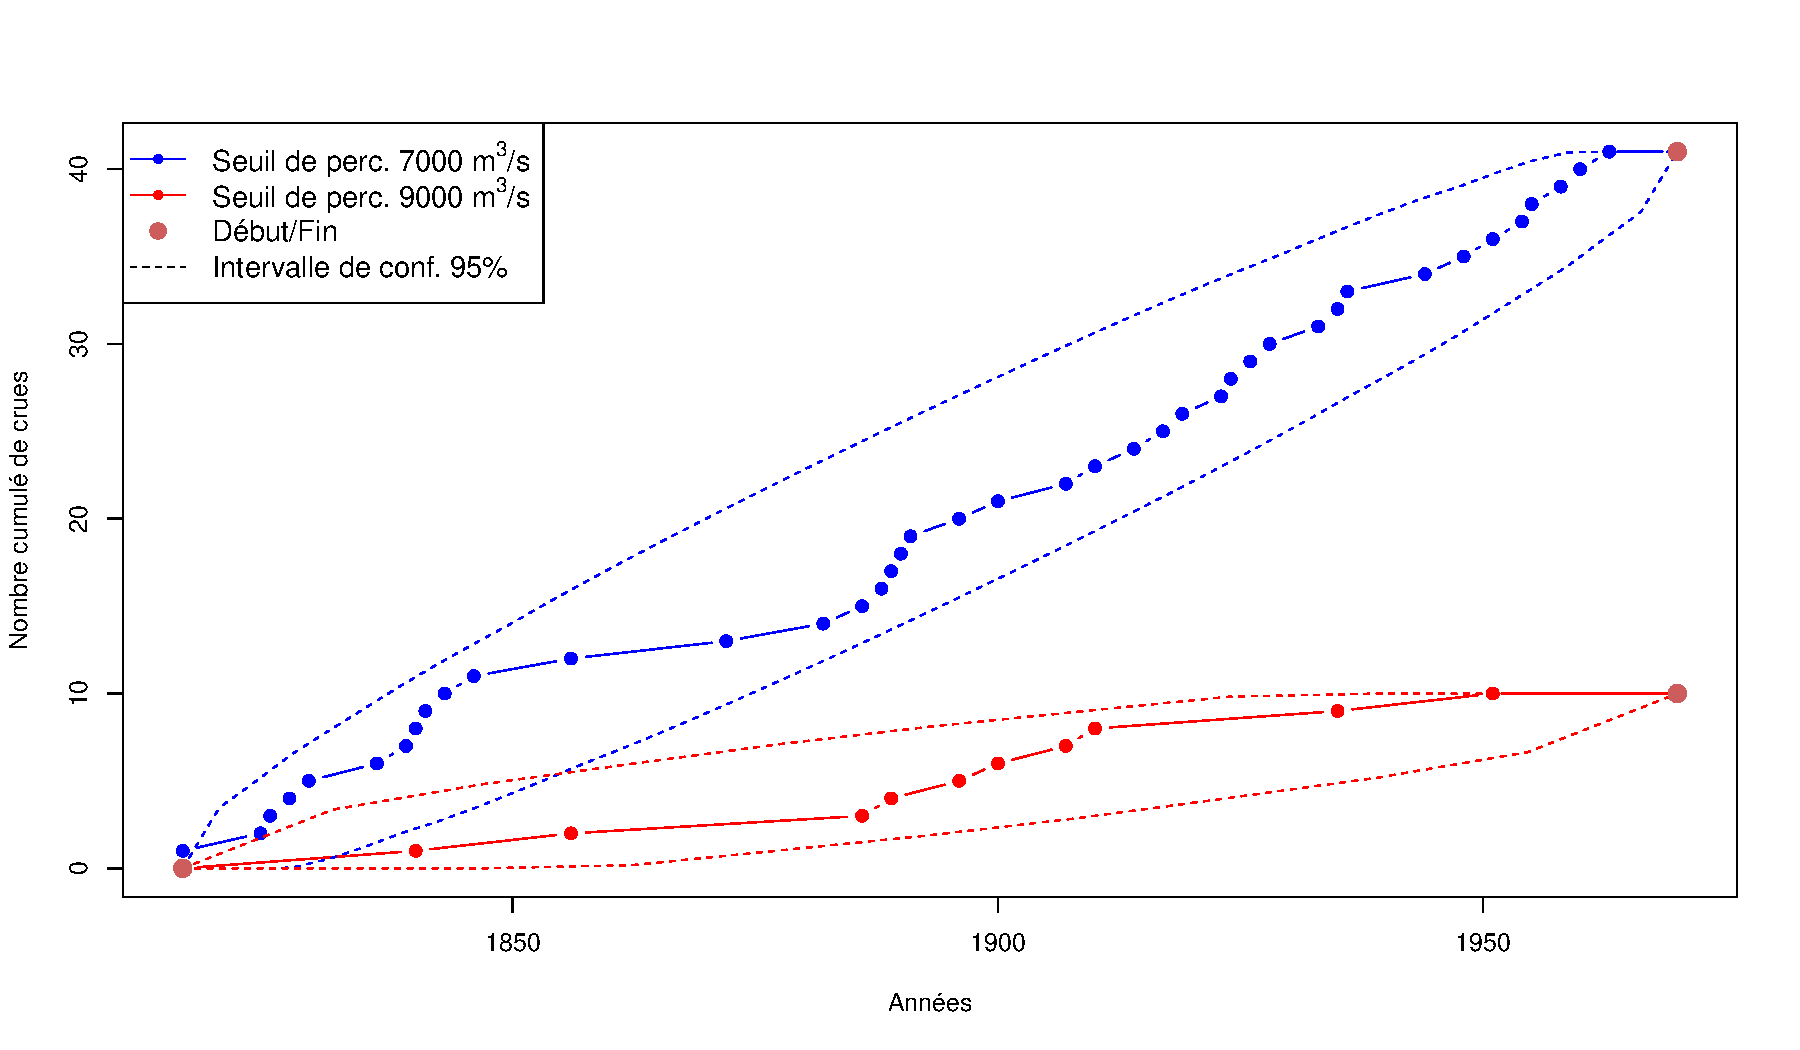
\includegraphics[width=.8\linewidth]{Figures/Poisson_Qrecent_FR.pdf}	
		\caption{Nombre de crues cumulé et intervalles de confiance à 95\% du processus de 						Poisson, pour deux échantillons d'occurrences de crues supérieures aux seuils $S3$ ou $S4$ à Pont de Beaucaire 							(1816-1969) }
		\label{fig:Poisson_Recent}
	\end{figure}
	
	
		
\FloatBarrier		
	
	
\section{Application aux crues du Rhône à Beaucaire}
\label{sec:applicationBcr}

	\paragraph{} Les 4 modèles décrits dans les sections précédentes (A, B, C et D) sont appliqués aux 4 échantillons de crues du Rhône à Beaucaire présentés dans le tableau \ref{tab:Echantillons}. Le modèle A fait l'hypothèse que le seuil de perception $S$ et la durée de la période historique $n$ sont parfaitement connus, tandis que dans le cas du modèle D, ces deux valeurs sont considérées incertaines. Le modèle B fait l'hypothèse que seul le seuil de perception $S$ est incertain, alors que pour le modèle C, seule la durée de la période historique $n$ est incertaine. Le modèle E suppose quant a lui que le débit des crues historique est connu et est contenu dans un intervalle de confiance, $S$ et $n$ sont alors supposés parfaitement connus. Pour les cinq modèles, l'incertitude des débits de la période continue est propagée. 
	
	\paragraph{} Les échantillons 1 et 2 représentent la combinaison des données pré-1816 décrites dans le chapitre 2 REF avec les données continues 1816-2020 estimées au chapitre 1 (REF). Les échantillons 3 et 4 sont basés sur les débits estimés au chapitre 1(REF) qui ont été dégradés pour créer artificiellement un échantillon mixte de données continues (1970-2020) et ponctuelles (1816-1969). Il s'agit ici de tailles d'échantillon plus usuelles et dont le seuil de perception et la durée de la période historique sont parfaitement connus, contrairement aux échantillons 1 et 2. Ainsi, pour les modèles faisant l'hypothèse que le seuil de perception et/ou la durée de la période historique sont inconnus, on jugera notamment la capacité du modèle à converger vers des valeurs acceptables. 
	
	\begin{table}[h]
		\centering
		\resizebox{\columnwidth}{!}{%
		%\begin{tabular}{|l|l|l|l|ll|l|l|}
		\begin{tabular}{|c|c|c|c|cc|c|c|}
		\hline
		\multicolumn{1}{|c|}{\multirow{2}{*}{n°}} &
		  \multirow{2}{*}{Période historique} &
		  \multirow{2}{*}{Période continue} &
		  \multirow{2}{*}{Seuil $S$ [m\textsuperscript{3}/s]} &
		  \multicolumn{2}{c|}{Nb. de crues $> S$} &
		  \multirow{2}{*}{A priori $S$ [m\textsuperscript{3}/s]} &
		  \multirow{2}{*}{A priori $t*$} \\ \cline{5-6}
		  
		 \multicolumn{1}{|c|}{} & & & & \multicolumn{1}{c|}{per. hist.} & per. cont. & & \\ \hline
		1 & 1500-1815 & 1816-2020 & 7000 & \multicolumn{1}{c|}{55} & 57 & $\mathcal{N}(7000,2000)$ & $\mathcal{U}(1111,1511)$ \\ \hline
		2 & 1500-1815 & 1816-2020 & 9000 & \multicolumn{1}{c|}{13} & 14 & $\mathcal{N}(9000,2000)$ & $\mathcal{U}(1129,1529)$ \\ \hline
		3 & 1816-1969 & 1970-2020 & 7000 & \multicolumn{1}{c|}{41} & 16 & $\mathcal{N}(7000,2000)$ & $\mathcal{U}(1316,1816)$ \\ \hline
		4 & 1816-1969 & 1970-2020 & 9000 & \multicolumn{1}{c|}{10} & 4 & $\mathcal{N}(9000,2000)$ & $\mathcal{U}(1340,1840)$ \\ \hline
		\end{tabular}%
		}
		\caption{Caractéristiques des échantillons de crues du Rhône à Beaucaire. $S$ désigne le seuil de perception et $t*$ la date de début de la période historique.}
		\label{tab:Echantillons}
	\end{table}		
	
	Les modèles B, C et D font l'hypothèse que $S$ et/ou $n$ sont inconnus, il faudra donc affecter une distribution a priori à ces paramètres. Ces distributions sont présentées dans le tableau \ref{tab:Echantillons} pour chacun des échantillons. Le but étant ici d'explorer les performances des modèles, les a priori seront très peu informatifs. L'a priori du seuil de perception $S$ (modèles B et D) est supposé Gaussien, avec pour moyenne la valeur connue ou supposée du seuil (soit $S3$ ou $S4$) et pour écart type 2000 m\textsuperscript{3}/s. Par souci de clarté, on ne parlera pas ici de la durée de la période historique $n$ mais de la date de début de la période historique $t*$ (la date de fin de la période historique étant ici parfaitement connue pour les 4 échantillons). La distribution a priori de $t*$ (modèles C et D) est supposée uniforme avec pour borne supérieure la date de la première crue de l'échantillon historique considéré, appelée $t_{k=1}$. Par définition, la période historique débute au plus tard à la date de cette première crue. La borne inférieure de la distribution uniforme sera fixée 400 ans avant la date de la première crue $t_{k=1}$ afin de représenter la méconnaissance de $t*$. 
			
	\FloatBarrier	
	
	\subsection{Résultats pour la période récente dégradée (1816-2020)}
	\label{subsec:ResultsArtif}
	
	\paragraph{} 
	Les 4 modèles décrits dans la section \ref{sec:MethodoCh3} ont été appliqués à l'échantillon 4 du tableau \ref{tab:Echantillons}. Les estimations pour les crues centennales et millénales sont présentées dans la figure \ref{fig:Barplot_Artif2}, dans laquelle les 4 modèles GEV-Binomiale sont comparés au modèle GEV (chapitre 1 (REF)) appliqué successivement à la chronique continue totale (1816-2020) et à la chronique continue dégradée (1970-2020).
	
	
	\begin{figure}[h]
		\centering
		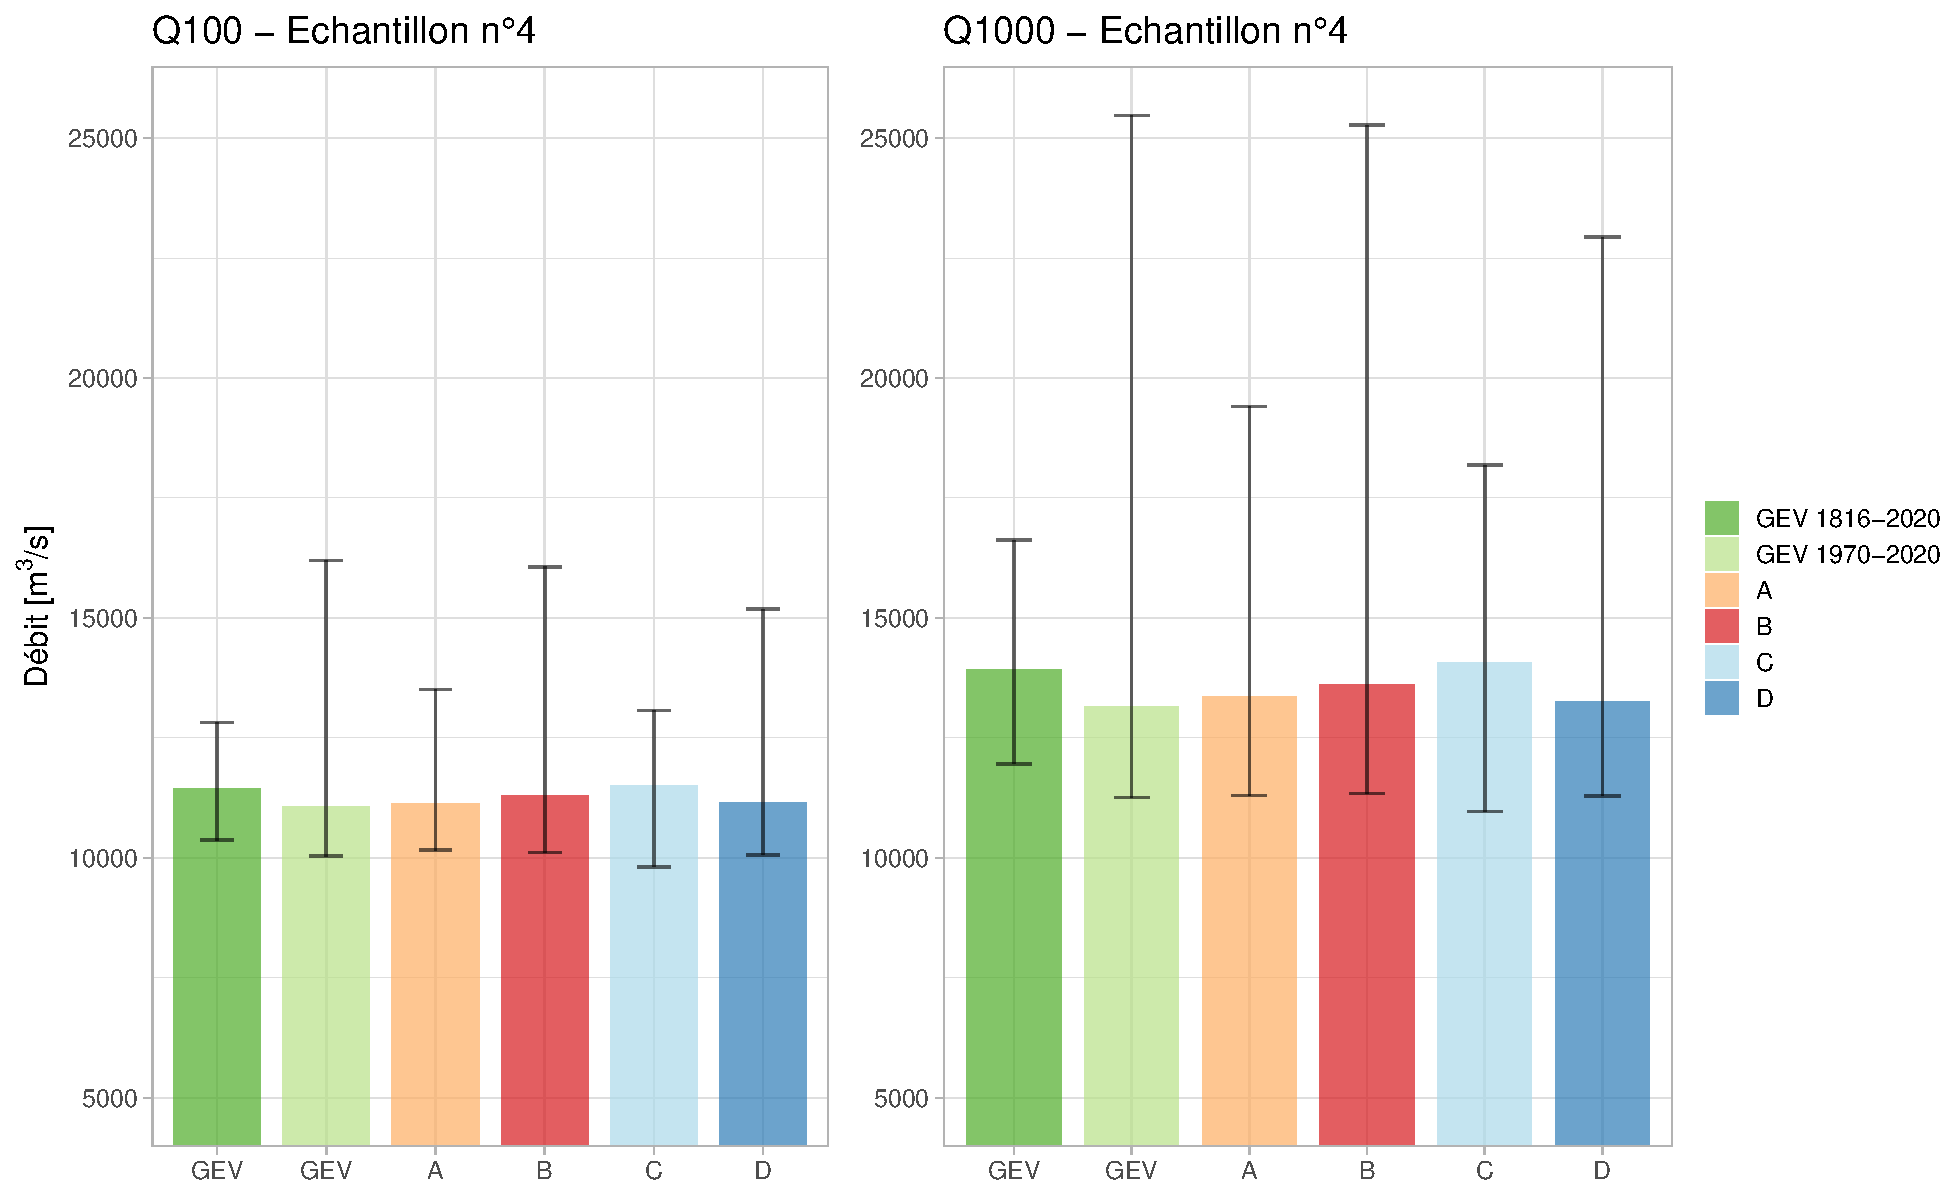
\includegraphics[width=.8\linewidth]{Figures/Barplots_QX_Artif2.pdf}	
		\caption{Estimations maxpost et incertitudes à 95\% pour Q100 et Q1000 pour 6 modèles appliqués à l'échantillon 4 (1816-2020 dégradé, $S4$)}
		\label{fig:Barplot_Artif2}
	\end{figure}

	\begin{table}[h]
	\centering
	\resizebox{\columnwidth}{!}{%
		\begin{tabular}{|c|c|c|c|c|c|c|c|c|c|c|}
		\hline
Modèle & Q100 [m\textsuperscript{3}/s] & uQ100 [m\textsuperscript{3}/s] & Q1000 [m\textsuperscript{3}/s] & uQ1000 [m\textsuperscript{3}/s] & $\xi$ & $u\xi$ & $S$ [m\textsuperscript{3}/s] & $uS$ [m\textsuperscript{3}/s] & $t*$ & $ut*$ \\ \hline
GEV 1816-2020 & 11451 & 687   & 13919 & 1351   & 0,058 & 0,044  & X    & X    & X    & X  \\ \hline
GEV 1970-2020 & 11076 & 2560  & 13154 & 6159   & 0,077 & 0,102  & X    & X    & X    & X  \\ \hline
A             & 11132 & 1189  & 13367 & 3019   & 0,062 & 0,088  & 9000 & X    & 1816 & X  \\ \hline
B             & 11302 & 2381  & 13622 & 5823   & 0,058 & 0,102  & 9163 & 729  & 1816 & X  \\ \hline
C             & 11517 & 779   & 14069 & 2057   & 0,041 & 0,083  & 9000 & X    & 1833 & 71 \\ \hline
D             & 11147 & 2018  & 13262 & 4837   & 0,074 & 0,096  & 9332 & 883  & 1785 & 107 \\ \hline
		\end{tabular}}
		\caption{Résultats maxpost et incertitudes des 6 modèles pour l'échantillon 4. Q100 et Q1000 représentent respectivement le débit des crues centennales et millénales, $\xi$ le paramètre de forme de la distribution GEV, $S$ le seuil de perception et $t*$ la date de début de la période historique. Les écarts type des distributions a posteriori sont représentés par les colonnes débutant par la lettre "u".}
		\label{tab:ResArtif2}
	\end{table}
	
	
	\paragraph{} On observe tout d'abord dans la figure \ref{fig:Barplot_Artif2} que l'incertitude du modèle GEV pour la période 1970-2020 est la plus importante de tous les modèles (avec un écart type de 6159 [m\textsuperscript{3}/s] contre 3019 [m\textsuperscript{3}/s] pour le modèle A dans le cas de la crue millénale). Cinquante années de données continues ne permettent pas d'obtenir une précision acceptable. Cela souligne l'intérêt de valoriser les données historiques dans une situation de ce type. Globalement, les estimations maxpost de l'ensemble des modèles sont proches. En revanche, les enveloppes d'incertitude sont très variables d'un modèle à l'autre, tout particulièrement pour les estimations millénales. 	
	
	\begin{figure}[h]
		\centering
		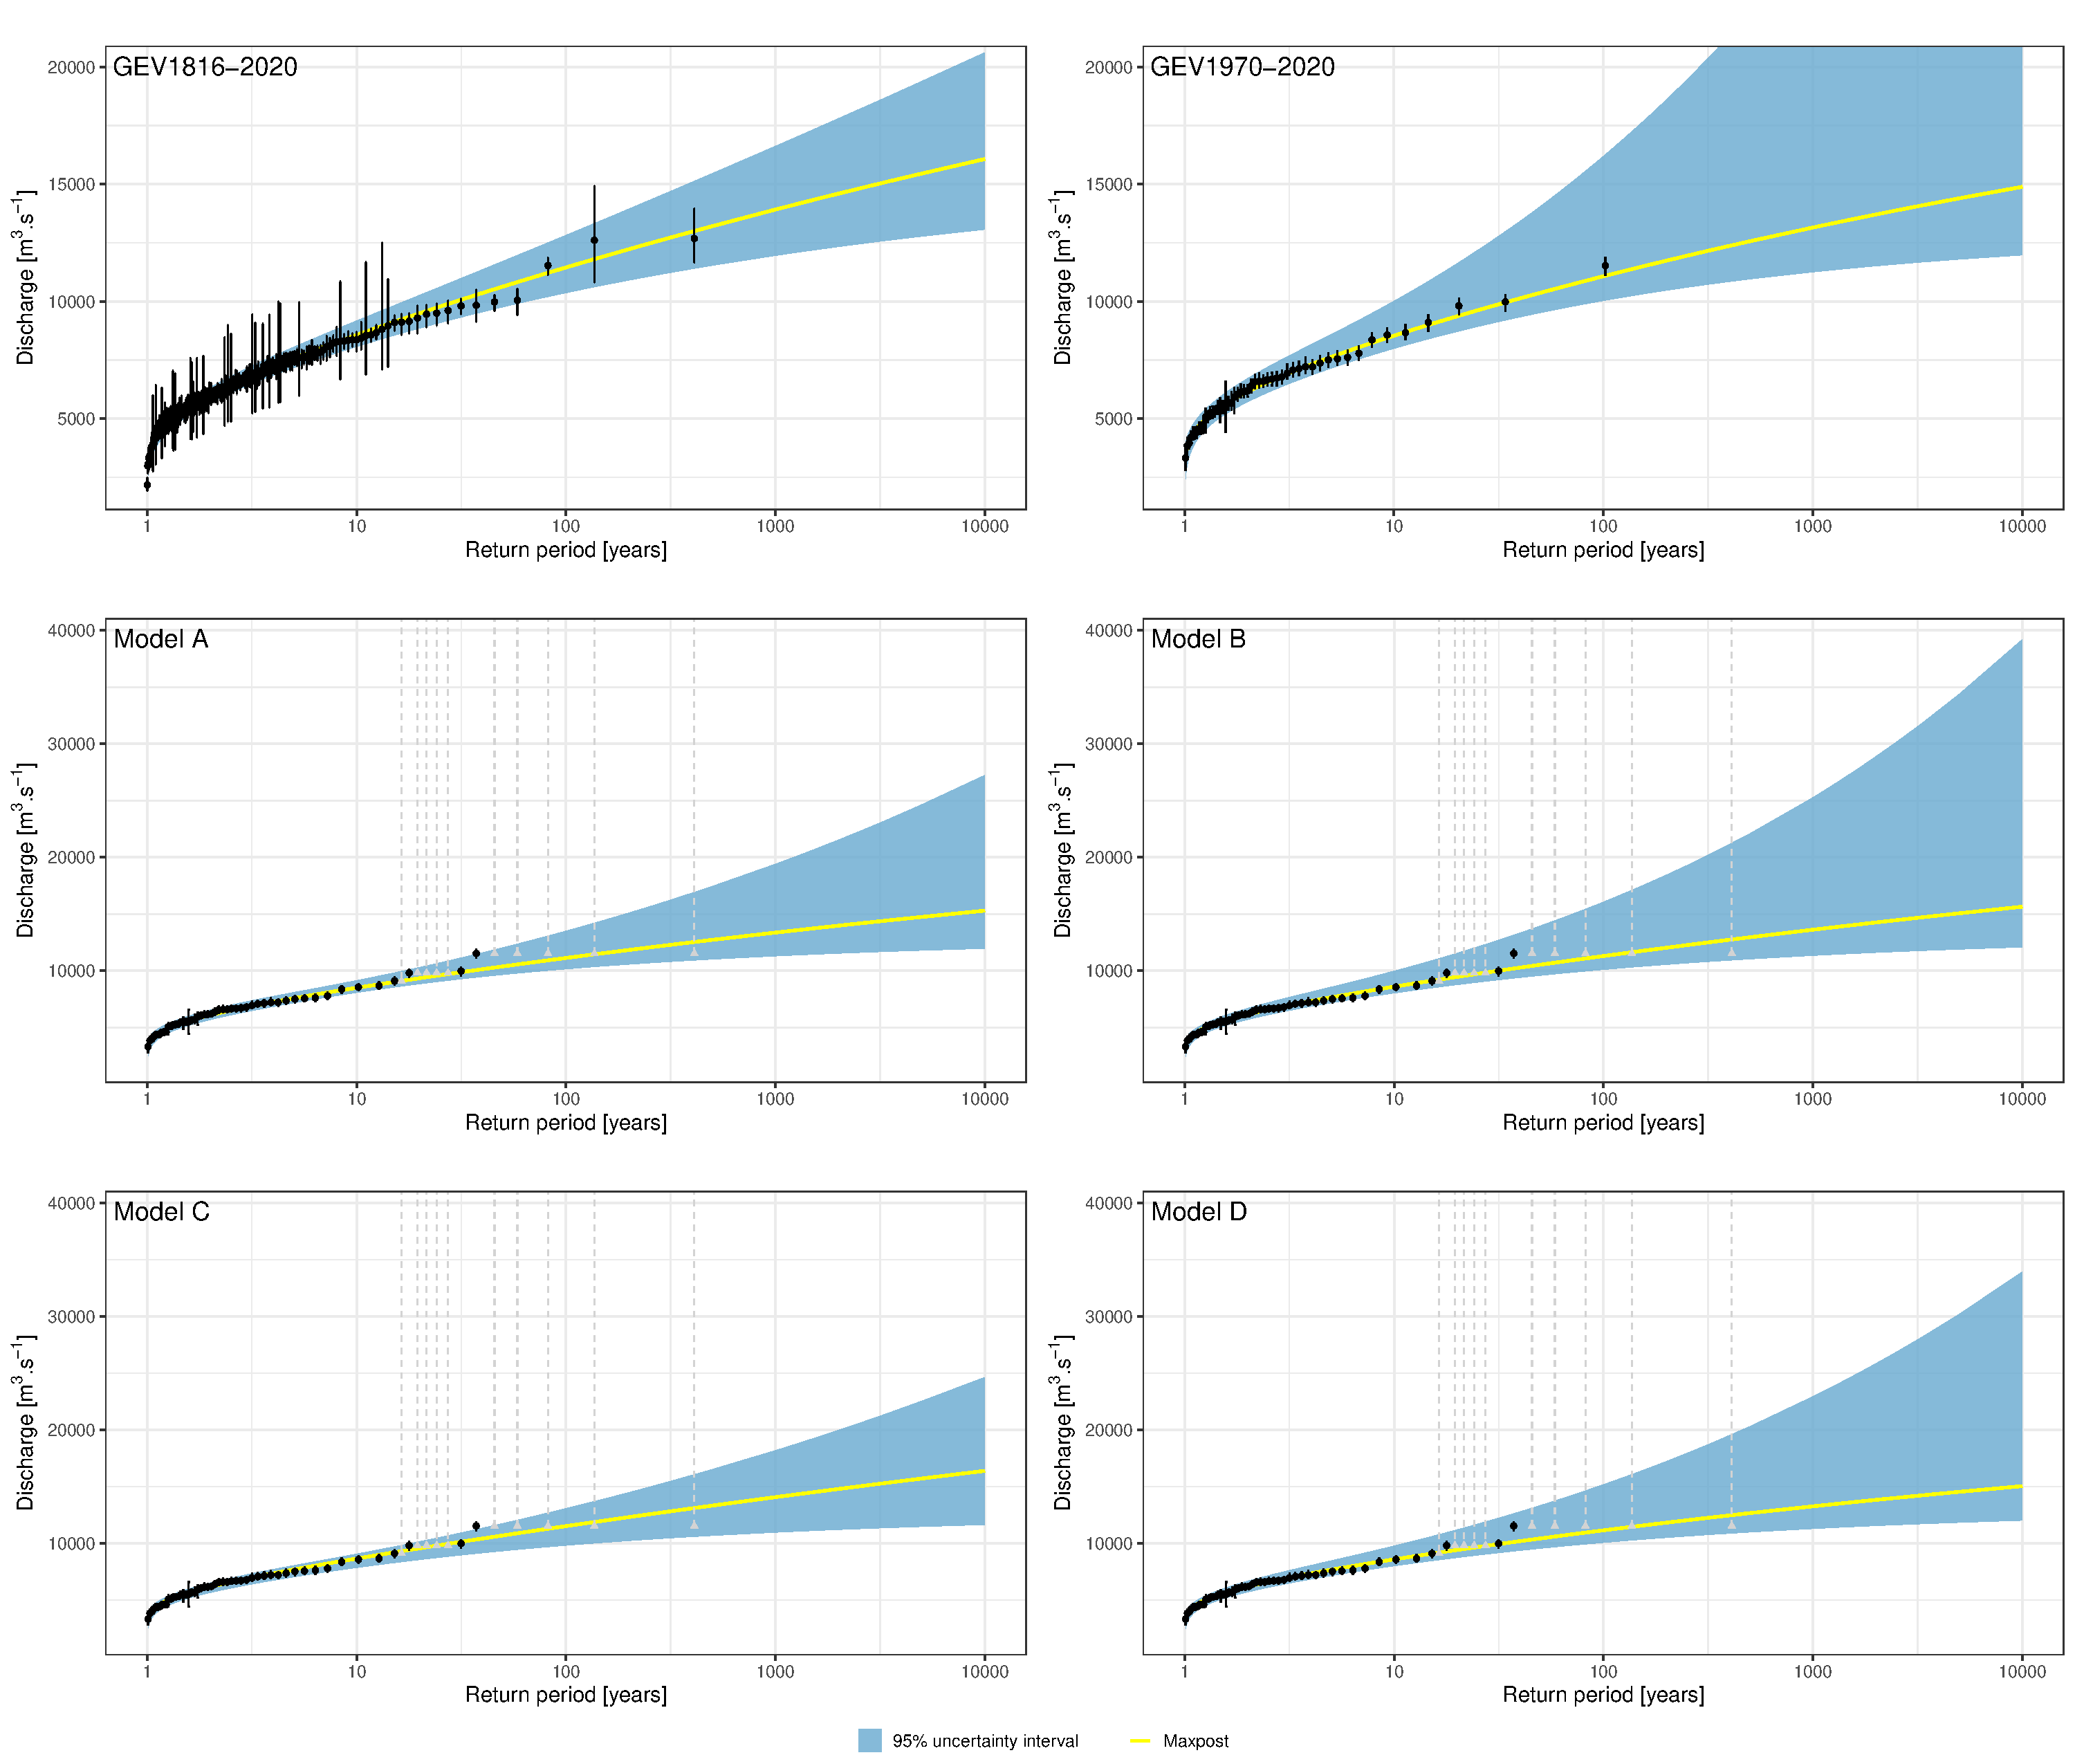
\includegraphics[width=\linewidth]{Figures/Quantiles_Artif2.pdf}	
		\caption{Quantiles de débit maximum annuel estimés par 6 modèles pour l'échantillon 4 (1816-2020 dégradé, $S4$). Les observations sont en noir pour la période continue (l'incertitude est également représentée) et en gris pour la période historique.}
		\label{fig:Quantiles_Artif2}
	\end{figure}
	
	\paragraph{} La figure \ref{fig:Quantiles_Artif2} présente l'ensemble des quantiles jusqu'à la crue décamillénale pour les 6 modèles. Ici, le rang des crues des deux périodes a été tiré aléatoirement comme décrit dans la section \ref{subsec:DistEmpirique}. Les estimations sont cohérentes avec les observations pour les 6 modèles. On remarque que l'incertitude croît rapidement au-delà la crue centennale pour les modèles B, D et GEV 1970-2020. 

\FloatBarrier
	
	\subsubsection{Quel est l'apport de l'utilisation des crues historiques pour une longueur de chronique "courante" ?}
	
	\paragraph{} Une durée de chronique continue trop courte devant la période de retour du quantile visé entraîne des résultats très incertains (GEV 1970-2020 en vert clair sur la figure \ref{fig:Barplot_Artif2}). La durée de la chronique continue (50 ans) est ici très petite devant la période de retour visée (100 ou 1000 ans). Si on se trouve dans l'impossibilité de reconstituer des débits en continu au-delà de 50 ans, on remarque que l'utilisation d'occurrences de crues historiques permet de réduire l'incertitude (modèle A en orange). Évidemment, l'utilisation de témoignages de crues ne permet pas d'atteindre la précision obtenue avec 200 ans de chronique continue (GEV 1816-2020 en vert foncé), mais l'incertitude obtenue s'en rapproche lorsque $S$ et $n$ sont connus. Pour les 6 modèles, une part de l'incertitude provient de l'estimation du paramètre de forme qui gouverne le comportement de la queue de distribution. On retrouve les valeurs a posteriori du paramètre de forme dans la figure \ref{fig:Shape_Artif2}. On notera que l'ensemble des estimations sont proches de zéro et légèrement positives, on se trouve donc dans le cas "queue légère" de la distribution GEV (cas "loi de Weibull"). Comme l'on peut s'y attendre, l'estimation de ce paramètre est plus précise dans le cas GEV 1816-2020. Les distributions a posteriori sont très proches pour les modèles A et C, tandis que distributions a posteriori des modèles B et D sont les plus larges (tableau \ref{tab:ResArtif2}). 
	
	\begin{figure}[h]
		\centering
		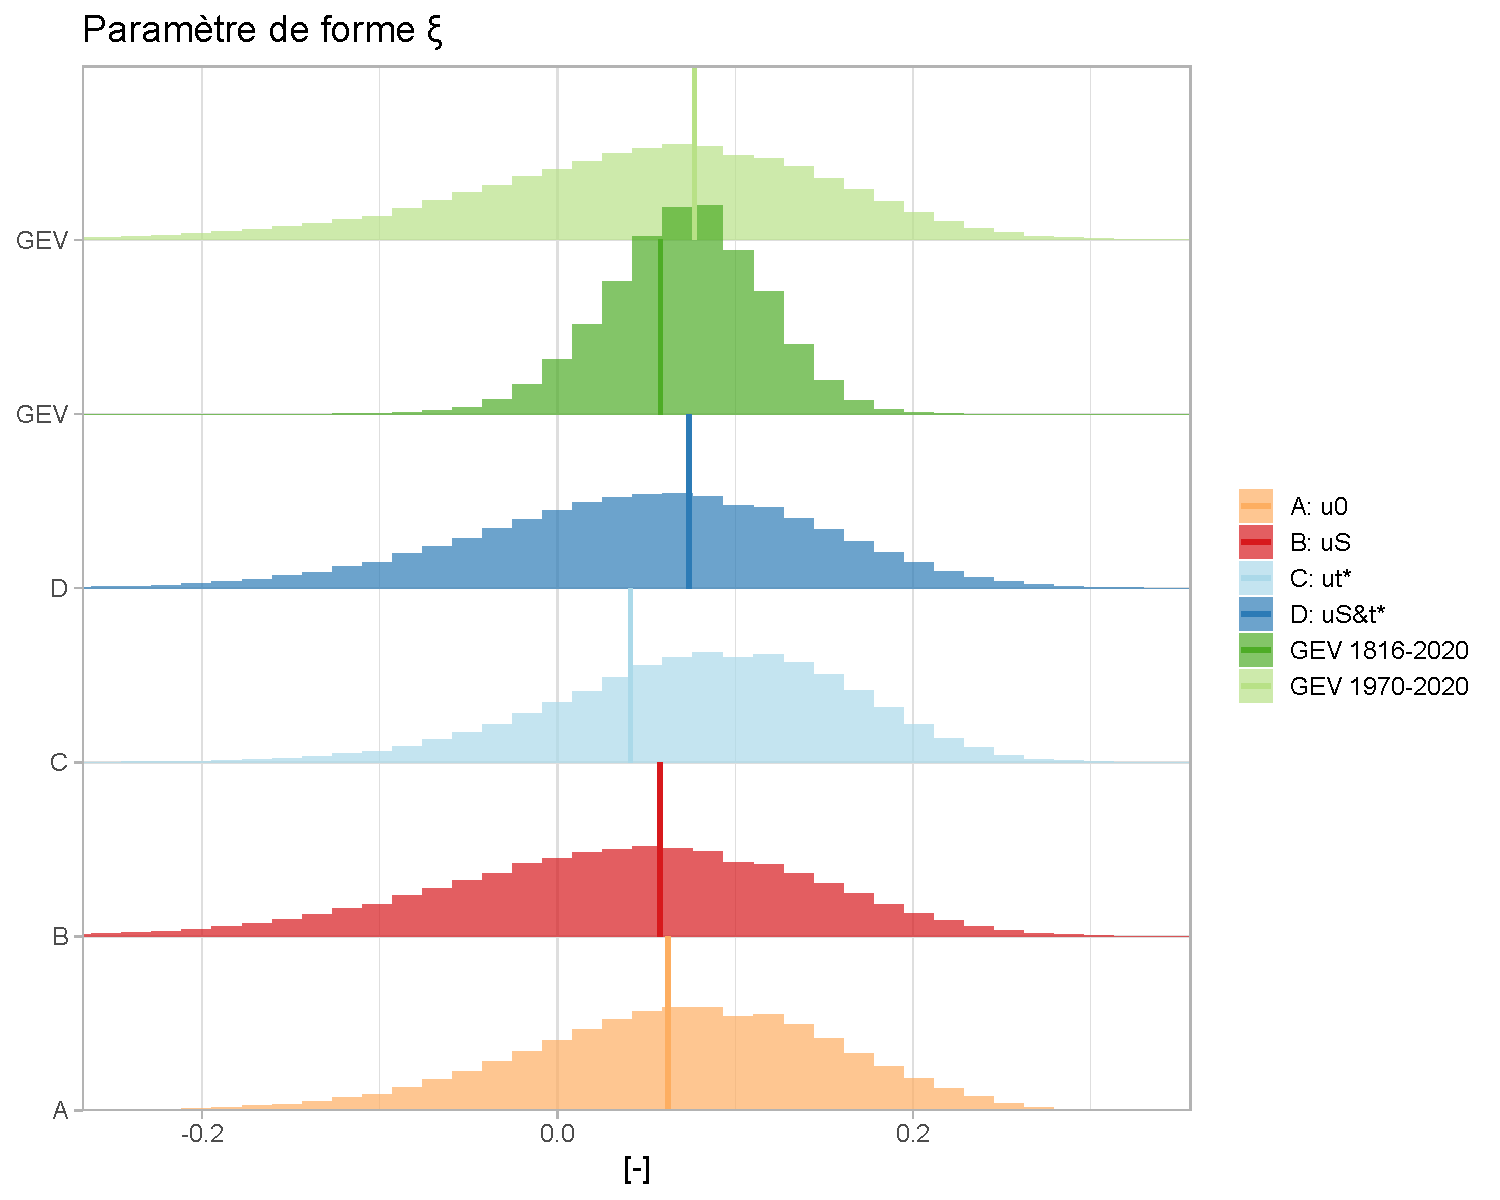
\includegraphics[width=.6\linewidth]{Figures/Shape_Artif2.pdf}	
		\caption{Distributions a posteriori du paramètre de forme de la distribution GEV des débits maximum annuels pour les 4 modèles estimés sur l'échantillon 4. Les estimations des modèles GEV sont également indiquées. Les droites verticales représentent les valeurs maxpost.}
		\label{fig:Shape_Artif2}
	\end{figure}

\FloatBarrier
	
	\subsubsection{Quel est l'impact de la méconnaissance du seuil de perception sur l'estimation des quantiles ?}
	
	\paragraph{} L'utilisation du modèle B reflète la méconnaissance du seuil de perception, celui-ci devenant alors un paramètre à part entière du modèle. Sur la figure \ref{fig:Barplot_Artif2}, on constate que l'incertitude autour des quantiles estimés par le modèle B est bien plus importante que pour le modèle A. La méconnaissance du seuil a donc des conséquences importantes sur les estimations. La vraie valeur du seuil de perception pour l'échantillon 4 est $S4$ = 9000 m\textsuperscript{3}/s. On retrouve les distributions a priori et a posteriori du seuil dans la figure \ref{fig:Params_Artif2}. On remarque que l'a posteriori pour le modèle B est proche de la vraie valeur, et que le modèle a effectivement permis d'améliorer la connaissance du seuil par rapport à l'a priori renseigné qui est ici très large : $\mathcal{N}(9000,2000)$. La valeur maxpost est de 9163 m\textsuperscript{3}/s soit une erreur relative de 2\%. Néanmoins, la méconnaissance de ce paramètre impacte grandement l'estimation des quantiles. L'écart type de la distribution de la crue millénale est pratiquement doublée par rapport au modèle A. Dans une situation plus réaliste, un a priori plus précis aurait pu être choisi afin de limiter cet impact. 
	
	 \begin{figure}[h]
		\centering
		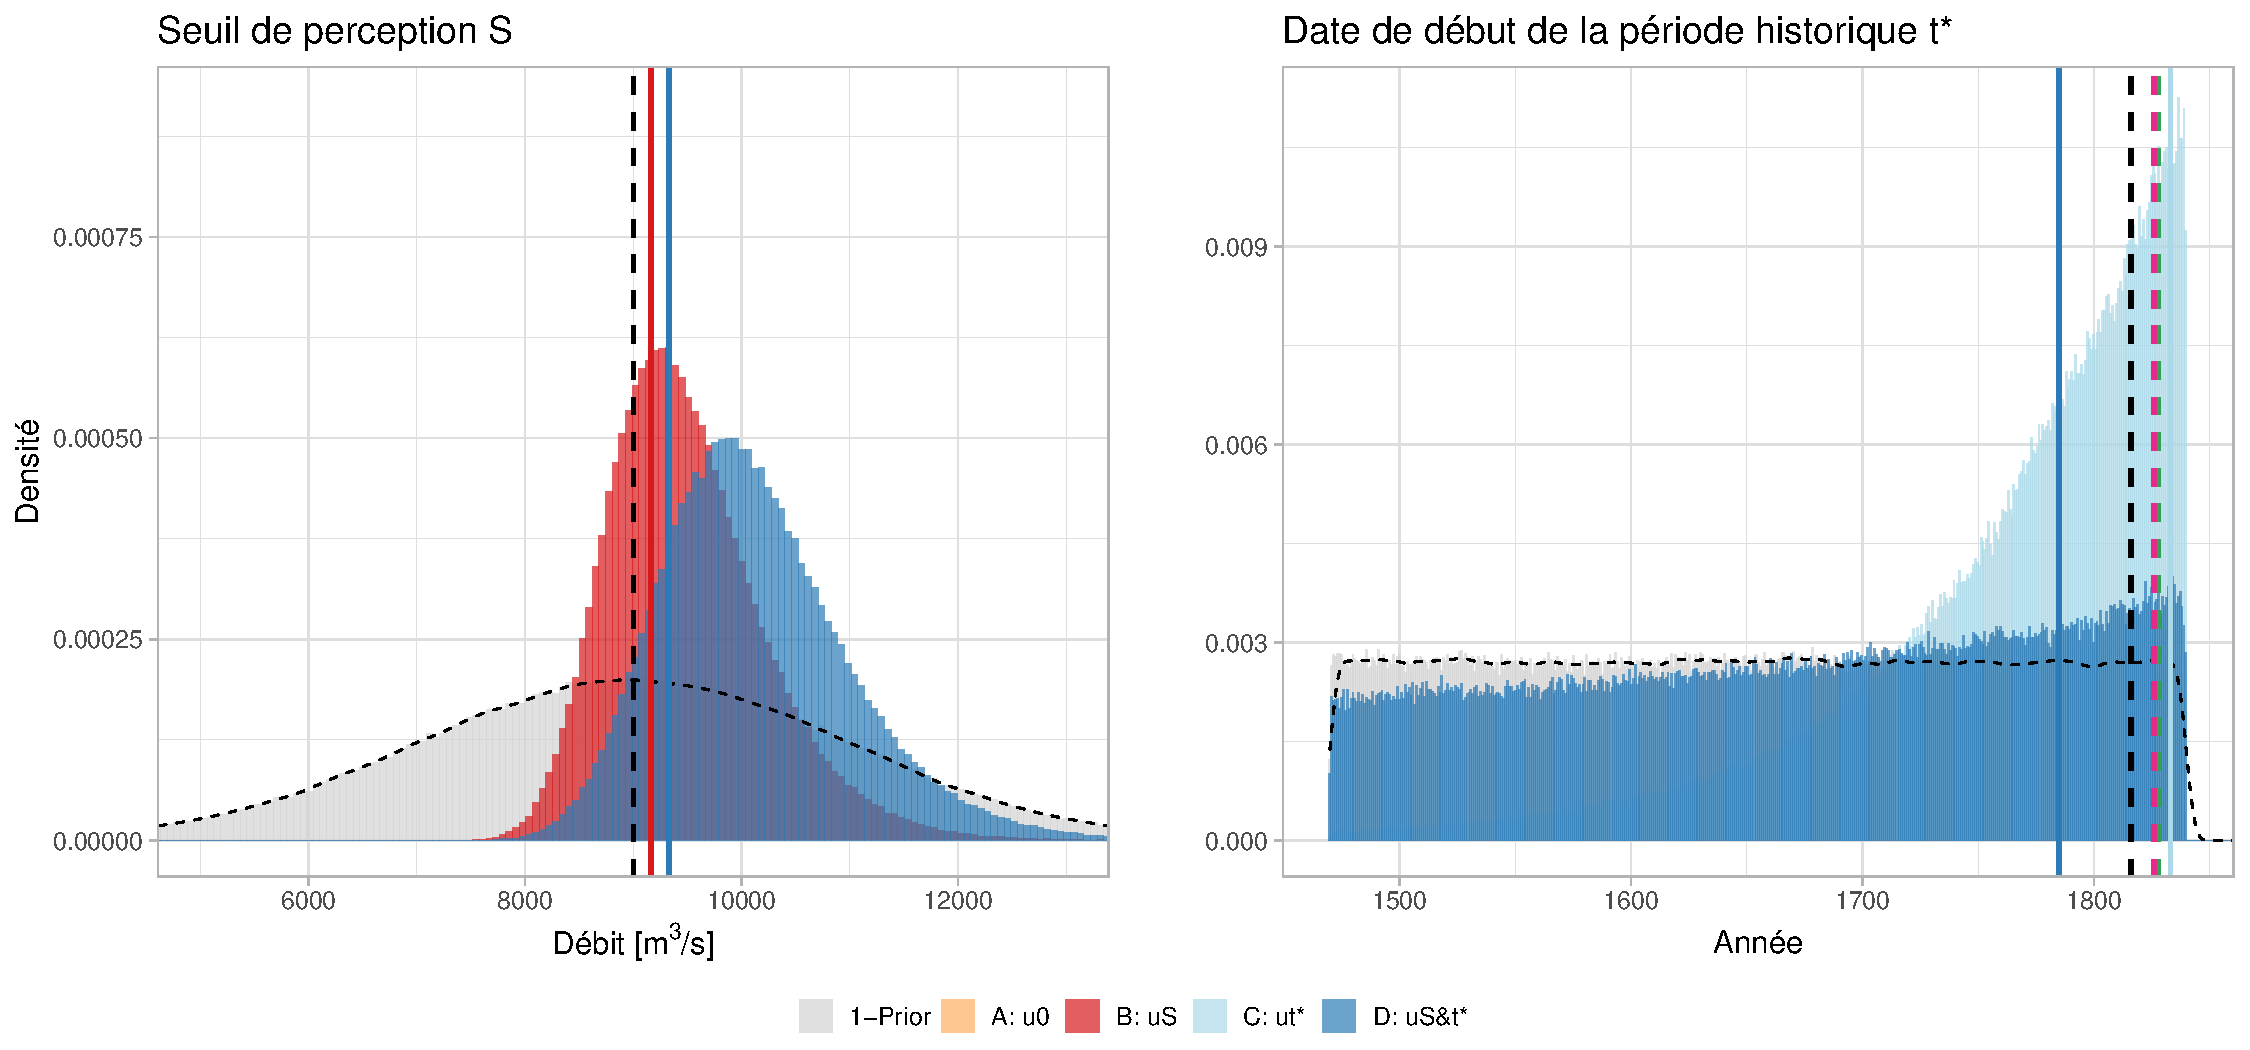
\includegraphics[width=.9\linewidth]{Figures/Params_Artif2.pdf}	
		\caption{Distributions a priori et a posteriori pour le seuil de perception (gauche) et la date de début de la période historique (droite). Les droites verticales pleines représentent l'estimation maxpost du paramètre pour chacun des modèles et les droites en pointillés noirs représentent les valeurs de référence. Les droites verticales en pointillés vert et rose représentent respectivement les estimations de $t*$ par la méthode de \cite{prosdocimi_german_2018} et la méthode de la période de retour du seuil $S$.}
		\label{fig:Params_Artif2}
	\end{figure}
	
	\subsubsection{Quel est l'impact de la méconnaissance de la durée de la période historique sur l'estimation des quantiles ?}	
	
	\paragraph{} Le modèle C permet de représenter la méconnaissance de la durée de la période historique, qui est l'un des deux paramètres de la loi binomiale utilisée ici pour modéliser le nombre d'occurrences de crues supérieures à un seuil. Sur la figure \ref{fig:Barplot_Artif2}, les estimations maxpost des quantiles pour le modèle C ont des valeurs légèrement supérieures aux estimations du modèle A. Cette légère sur-estimation provient d'une durée de période historique sous-estimée par le modèle, visible sur la figure \ref{fig:Params_Artif2} (droite). En effet, la date maxpost est l'année 1833, alors que la chronique débute réellement en 1816. Cette sur-estimation de 16 ans peut s'expliquer par une fréquence des crues supérieures au seuil $S4$ plus importante au cours de la période continue (4 crues / 50 ans = 0.08 crues/an) qu'au cours de la période historique (10 crues / 153 ans = 0.065 crues/an). Ce déséquilibre reflète l'existence de phases durant lesquelles la fréquence d'occurrence des crues oscille malgré le fait qu'aucune non-stationnarité des données n'ait été détectée par les tests à la section (REF). L'impact de ces phases est exacerbé par des longueurs de chronique trop petites devant la durée de ces oscillations. 
	\paragraph{} L'incertitude autour des quantiles estimée par le modèle C est très similaire à celle estimée par le modèle A (figure \ref{fig:Barplot_Artif2}), de même que la distribution du paramètre de forme (figure \ref{fig:Shape_Artif2}), et ce malgré un a priori très peu informatif pour la date de début de la période historique : $\mathcal{U}(1340,1840)$. Une forte méconnaissance de la durée de la période historique n'a donc que peu d'impact sur la précision de l'estimation des quantiles, contrairement à la méconnaissance du seuil de perception.
	
	\subsubsection{Quel est l'impact de la méconnaissance du seuil de perception et de la durée de la période historique sur l'estimation des quantiles ?}	
	
	\paragraph{} Représenter la méconnaissance autour de $S$ et $n$ en même temps dans le modèle fréquentiel paraît être la solution la plus raisonnable dans certains cas, notamment pour des événements très anciens et mal connus. Le modèle D est ici utilisé à cet effet. Les quantiles maxpost estimés dans la figure \ref{fig:Barplot_Artif2} pour le modèle D semblent cohérents avec les valeurs de référence. En revanche, la largeur de l'intervalle de confiance est importante et se situe entre celle du modèle B et du modèle C. Même si l'estimation est plus précise que celle du modèle GEV sur l'échantillon 1970-2020, elle reste imprécise pour la crue millénale. L'observation des paramètres a posteriori sur la figure \ref{fig:Params_Artif2} permet de comprendre l'origine de cette large incertitude. La distribution du seuil de perception, bien que centrée a proximité de la vraie valeur (maxpost à 9331 m\textsuperscript{3}/s), est très large (écart type = 883 m\textsuperscript{3}/s). Le seuil de perception parait ici un peu moins bien estimé que par le modèle B (écart type = 729 m\textsuperscript{3}/s). La date de début de la période historique est elle encore plus difficilement estimée, notamment en comparaison avec l'estimation du modèle C. On remarque que la distribution a posteriori est pratiquement aussi large que celle de l'a priori, même si elle marque un maximum non loin de la vraie valeur (l'année 1816). Cependant, les quantiles présentent une plus faible incertitude pour le modèle D que pour le modèle D. Cela provient de corrélations entre les paramètres qui peut être observée sur la figure \ref{fig:ScatterD_Artif2}. On remarque notamment une assez bonne corrélation entre la durée de la période historique $n$ et le seuil de perception $S$, ainsi qu'entre le seuil de perception et le paramètre de forme $xi$. Il est donc complexe d'identifier ces paramètres séparément. Une élicitation plus précise de leurs a priori sera certainement nécessaire.
	
	\begin{figure}[h]
		\centering
		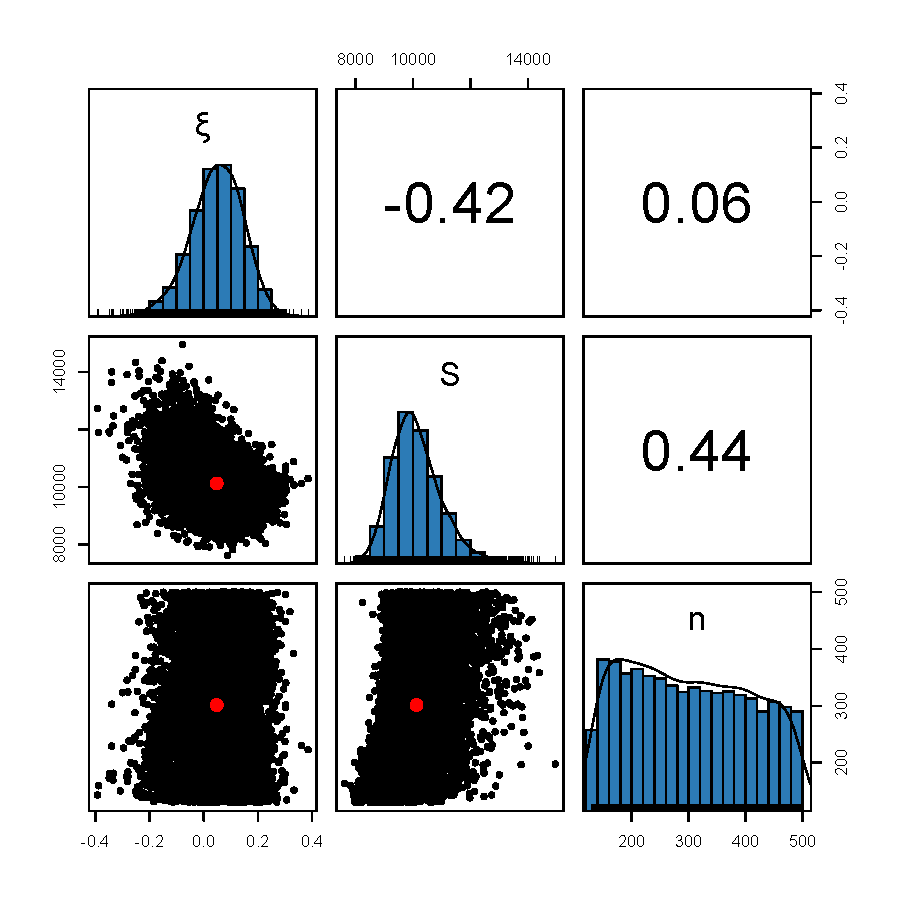
\includegraphics[width=.7\linewidth]{Figures/ScatterD_Artif2.pdf}
		\caption{Scatterplots des distributions a posteriori de trois paramètres du modèle D pour l'échantillon 4 : le paramètre de forme $\xi$ (sans unité), le seuil de perception $S$ (en m\textsuperscript{3}/s) et la durée de la période historique $n$ (en années). Les nombres inscrits dans les cases supérieures correspondent aux corrélations entre les paramètres.}
		\label{fig:ScatterD_Artif2}
	\end{figure}
		
\FloatBarrier

	\subsubsection{Quel est l'apport de la connaissance du débit des crues historiques ?}

	\paragraph{} Les modèles A, B, C et D n'utilisent que l'information du nombre de dépassements $k$ d'un seuil de perception $S$ pendant une durée $n$. Le débit des crues historiques ayant dépassé le seuil est donc ignoré. Le modèle E permet de prendre en compte cette donnée de débit ainsi que l'incertitude correspondant à chaque crue. Il a été appliqué à l'échantillon 4 du tableau \ref{tab:Echantillons} en considérant l'incertitude des débits de la période historique (1816-1969) calculée au chapitre 1 (REF).
	
	
	\begin{figure}[h]
		\centering
		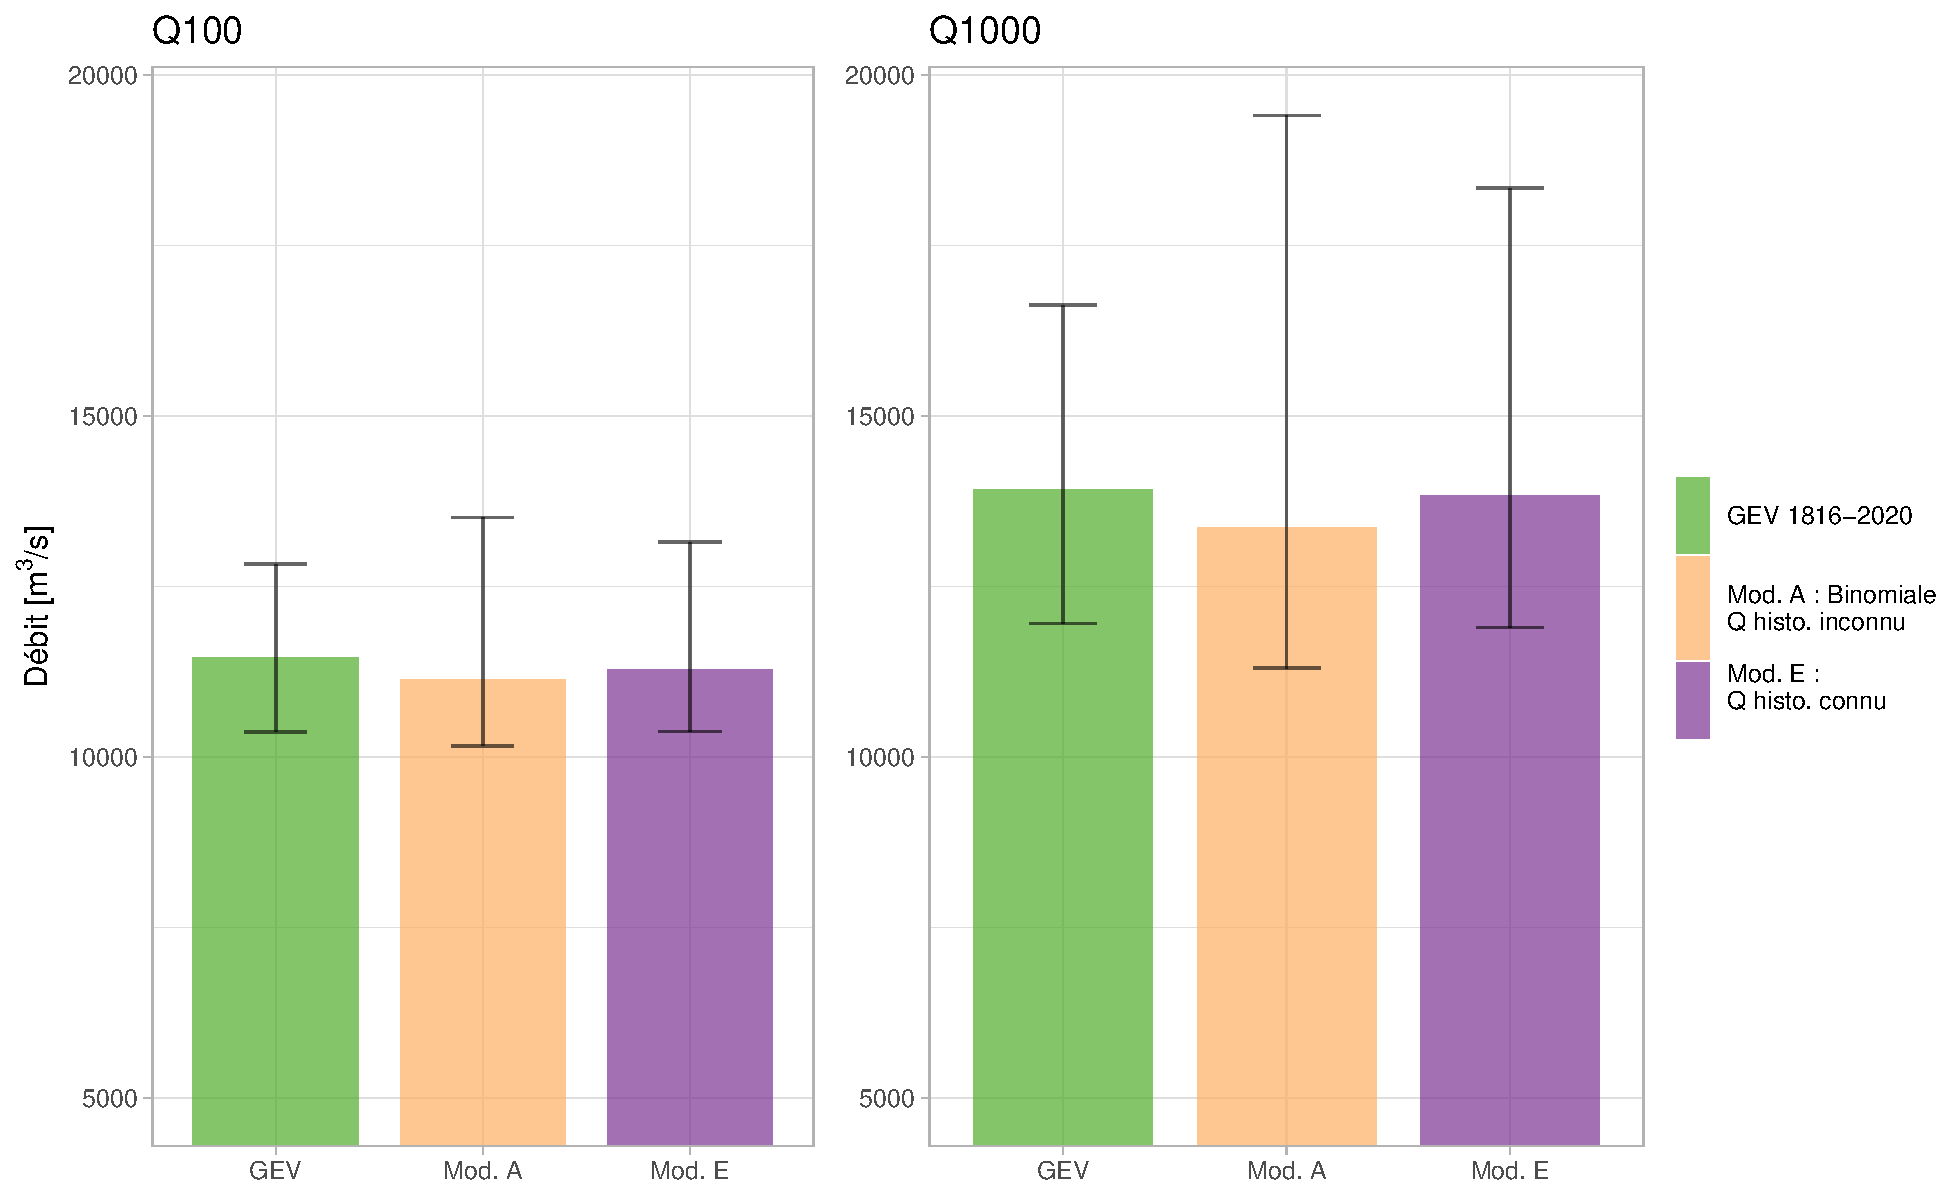
\includegraphics[width=.8\linewidth]{Figures/Barplots_QX_censure.pdf}
		\caption{Estimations maxpost et incertitudes à 95\% pour Q100 et Q1000 pour 3 modèles appliqués à l'échantillon 4 (1816-2020 dégradé, $S4$). Le modèle A n'utilise que le nombre de dépassements du seuil de perception, alors que le modèle E considère le débit des crues historique (et son incertitude) ayant dépassé le seuil $S$.}
		\label{fig:CensureArtif}
	\end{figure}
	
	\begin{table}[h]
		\centering
%		\resizebox{\columnwidth}{!}
		\caption{Résultats maxpost et incertitudes pour trois modèles appliqués à l'échantillon 4. Q100 et Q1000 représentent respectivement le débit des crues centennales et millénales. Les écarts type des distributions a posteriori sont représentés par les colonnes débutant par la lettre "u". }
		\label{tab:ResCensure}
	\end{table}
	
	\paragraph{}
	Les résultats sont présentés dans la figure \ref{fig:CensureArtif} et le tableau \ref{tab:ResCensure}. On constate une diminution de l'incertitude d'environ 25\% autour du Q1000 pour le modèle E (avec un écart type de 2255 [m\textsuperscript{3}/s] pour Q1000) par rapport au modèle binomial A (écart type de 3013 [m\textsuperscript{3}/s] pour Q1000). En revanche, l'incertitude du modèle E reste environ 65\% supérieure à celle du modèle GEV 1816-2020 pour Q1000. La connaissance du débit des crues historiques, bien qu'elle ne soit pas une condition nécessaire à l'utilisation de données pré-enregistrements systématiques, permet donc de réduire l'incertitude autour des quantiles extrêmes. Cette incertitude reste en revanche supérieure à celle du modèle GEV pour lequel le débit maximum annuel de toutes les années de l'échantillon (historique + continu) est connu.	

	\subsubsection{Discussion intermédiaire}
	
	\paragraph{} L'utilisation des modèles décrits dans la section \ref{sec:MethodoCh3} sur un échantillon artificiellement dégradé et dont les caractéristiques sont parfaitement connues permet d'évaluer la performance des modèles et l'impact de la méconnaissance du seuil de perception $S$ et de la durée de la période historique $n$ sur l'estimation des quantiles extrêmes. On constate en observant les résultats que la méconnaissance du seuil de perception a un plus fort impact sur l'incertitude des résultats que la méconnaissance de la durée de la période historique. Même si les distributions a posteriori du seuil de perception pour les modèles B et D sont centrées a proximité de la vraie valeur (9000 m\textsuperscript{3}/s), l'incertitude résultant de la détermination du seuil a un fort impact sur l'incertitude des quantiles. En revanche, l'estimation de la durée de la période historique dans le cas des modèles C et D semble elle aussi relativement peu précise, mais n'impacte que peu l'incertitude des résultats si on compare ces derniers à ceux du modèle A. Cela est dû à des corrélations entre paramètres (figure \ref{fig:ScatterD_Artif2}) qui entraînent une réduction de l'incertitude finale.
	 
	\paragraph{} Ces premiers résultats démontrent que l'incertitude des quantiles peut être sous-estimée	lorsque l'on considère seuil de perception et durée de période historique comme étant bien connus alors que ce n'est pas le cas. Les modèles utilisés ici permettent de prendre en compte cette méconnaissance dans l'estimation des quantiles extrêmes. On pourra par la suite les appliquer au cas réel de l'échantillon de crues de la période 1500-2020 à Beaucaire, dont le seuil de perception et la durée de période historique ne sont pas connus précisément. Si les a priori utilisés jusqu'ici étaient peu informatifs afin de comprendre les performances du modèle, ils devront être élicités plus précisément par la suite afin d'obtenir des résultats qui reflètent davantage la connaissance/méconnaissance du seuil de perception et de la durée de la période historique.
		
	\paragraph{} Enfin, la comparaison du modèle A pour lequel seul le nombre de dépassements du seuil de perception est connu avec le modèle E pour lequel le débit des crues historiques est connu (ainsi que l'incertitude autour de ces débits) a permis de démontrer l'intérêt de reconstituer le débit des crues historiques. Néanmoins, ces résultats ne sont valables que pour le seuil de perception $S4$ utilisé ici. Plusieurs études (notamment \citet{stedinger_flood_1986} et \citet{payrastre_usefulness_2011}) ont démontré que l'écart d'incertitude entre les résultats de ces deux types de modèles tendait à se réduire à mesure que la période de retour du seuil de perception tendait vers environ 50 ans, jusqu'à devenir nul au delà de cette magnitude. Cette affirmation encourage donc l'utilisation du nombre de dépassements d'un seuil de perception lorsqu'il n'est pas possible d'avoir de meilleure information sur la période historique. Au demeurant, les résultats de cette section mettent en garde sur le fait de supposer que le seuil de perception est parfaitement connu et dans une moindre mesure que la durée de la période historique est connue lorsque ce n'est pas le cas.
	
	\subsection{Application à la période 1500-2020}
	\label{subsec:Results1500}
	
	\paragraph{} Les modèles A, B, C et D de la section \ref{sec:MethodoCh3} ont été appliqués à l'échantillon 2 (1500-2020, seuil $S4$), les résultats sont présentés dans la figure \ref{fig:BarplotC4} et sont comparés au modèle GEV sur l'échantillon continu 1816-2020. Sans surprise, on observe des résultats moins incertains que pour l'échantillon dégradé (figure \ref{fig:Barplot_Artif2}). L'incertitude des résultats des modèles GEV-Binomiale est au moins équivalente à celle de la référence (GEV 1816-2020), voire plus faible pour les modèles supposant un seuil de perception connu (A et C).

	\begin{figure}[h]
		\centering
		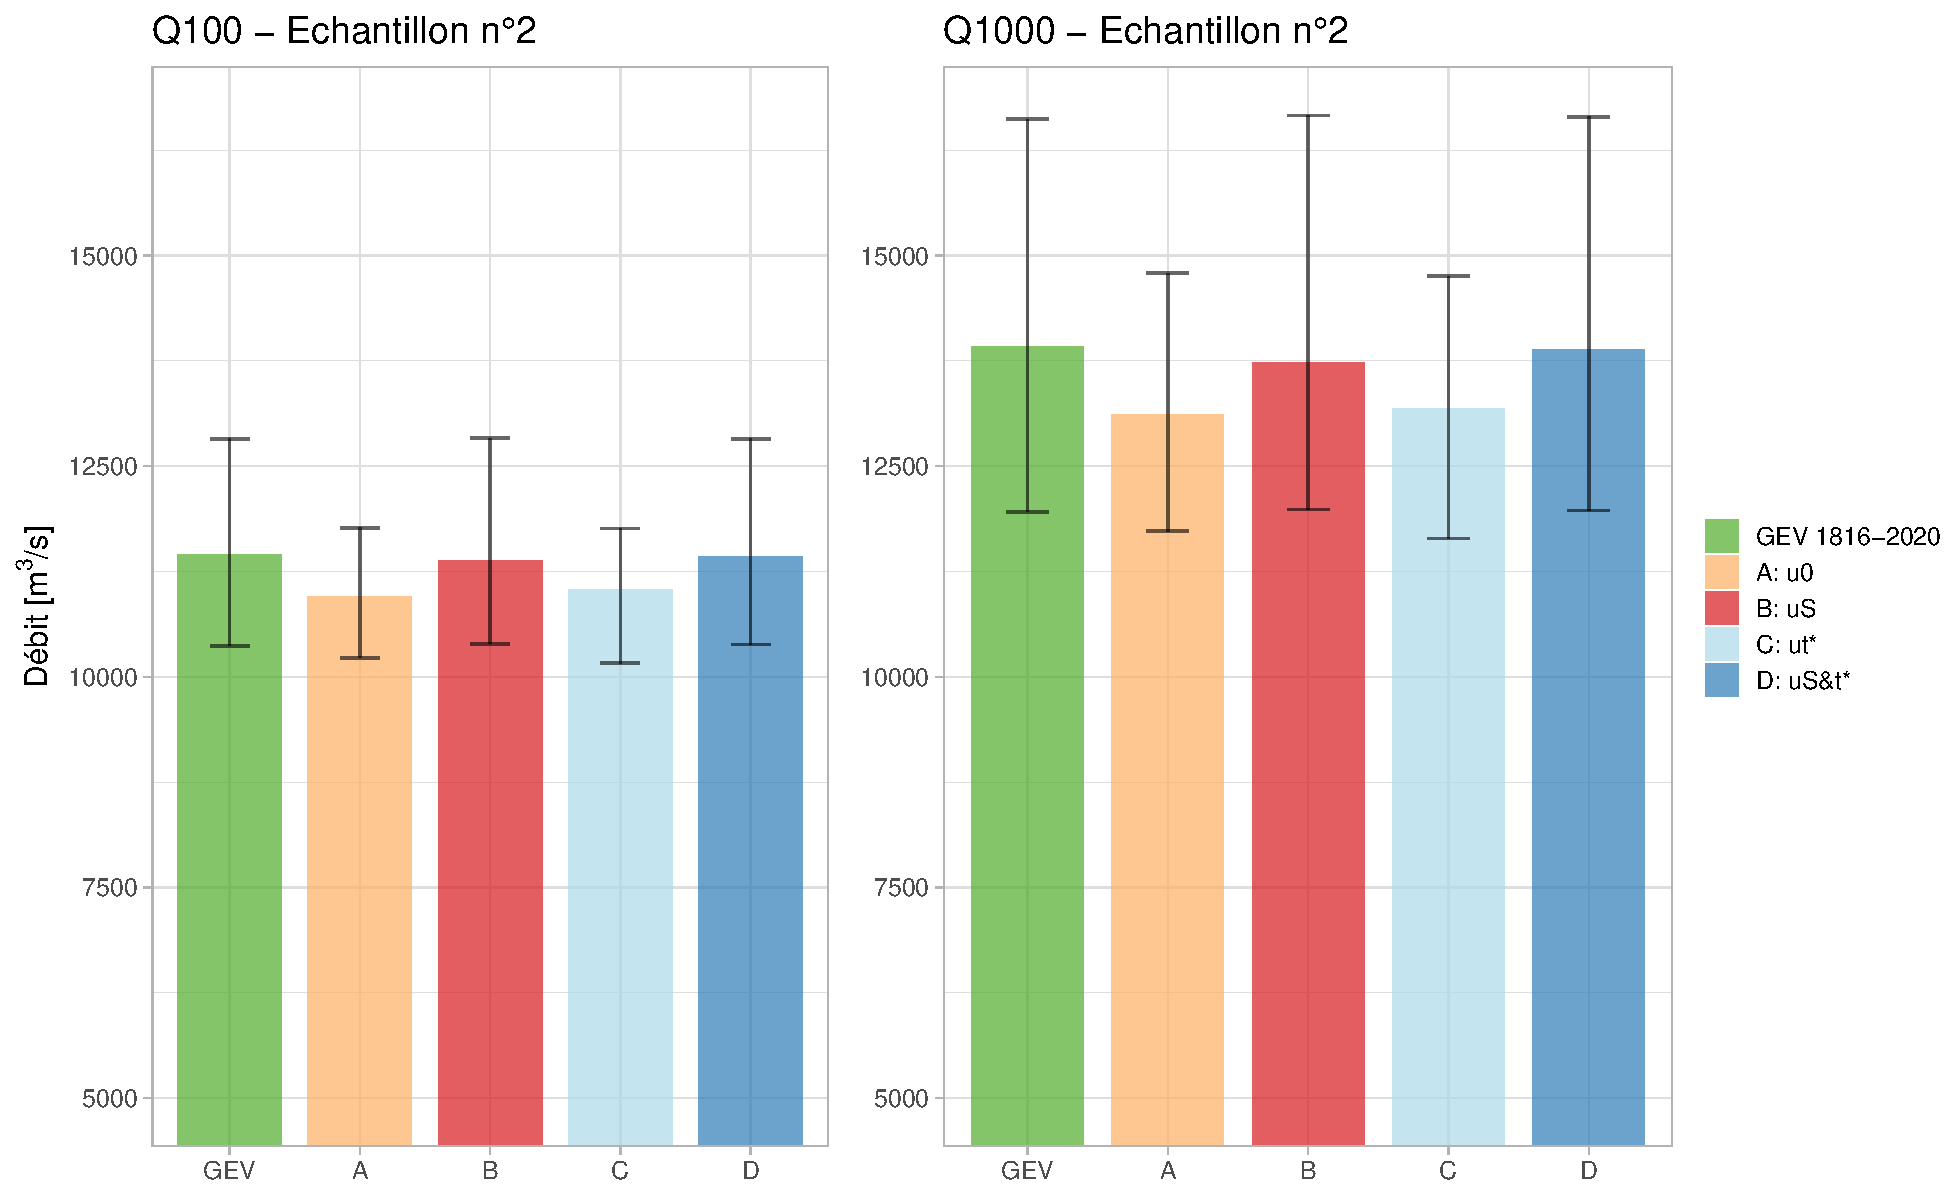
\includegraphics[width=.8\linewidth]{Figures/Barplots_QX_C4.pdf}
		\caption{Estimations maxpost et incertitudes à 95\% pour Q100 et Q1000 par 5 modèles différents pour l'échantillon 2 (1500-2020, $S4$)}
		\label{fig:BarplotC4}
	\end{figure}
	
		\begin{table}[h]
	\centering
	\resizebox{\columnwidth}{!}{%
		\begin{tabular}{|c|c|c|c|c|c|c|c|c|c|c|}
		\hline
Modèle & Q100 [m\textsuperscript{3}/s] & uQ100 [m\textsuperscript{3}/s] & Q1000 [m\textsuperscript{3}/s] & uQ1000 [m\textsuperscript{3}/s] & $\xi$ & $u\xi$ & $S$ [m\textsuperscript{3}/s] & $uS$ [m\textsuperscript{3}/s] & $t*$ & $ut*$ \\ \hline
GEV 1816-2020 & 11451 & 687   & 13919 & 1351   & 0,058 & 0,044  & X    & X    & X    & X \\ \hline
A             & 10977 & 391   & 13149 & 816    & 0,073 & 0,038  & 9000 & X    & 1500 & X \\ \hline
B             & 11438 & 698   & 13875 & 1391   & 0,06  & 0,044  & 9628 & 504  & 1500 & X \\ \hline
C             & 10975 & 395   & 13139 & 809    & 0,074 & 0,038  & 9000 & X    & 1527 & 44 \\ \hline
D             & 11336 & 745   & 13721 & 1467   & 0,061 & 0,044  & 9613 & 551  & 1529 & 62 \\ \hline
		\end{tabular}}
		\caption{Résultats maxpost et incertitudes des 5 modèles pour l'échantillon 2. Q100 et Q1000 représentent respectivement le débit des crues centennales et millénales, $\xi$ le paramètre de forme de la distribution GEV, $S$ le seuil de perception et $t*$ la date de début de la période historique. Les écarts type des distributions a posteriori sont représentés par les colonnes débutant par la lettre "u".}
		\label{tab:ResC4}
	\end{table}
	
	\paragraph{} Les distributions a posteriori de $S$ et $t*$ sont présentées dans la figure \ref{fig:Params_C4}. Ces distributions sont similaires à celles observées pour l'échantillon 4 pour lequel les a priori étaient les mêmes. Le modèle estime un seuil de perception supérieur à la valeur de 9000 m\textsuperscript{3}/s (modèles B et D, tableau \ref{tab:ResC4}), ainsi qu'une date de début de la période historique plus récente que la valeur supposée de 1500 (modèles C et D, tableau \ref{tab:ResC4}). Cette tendance exprimée par les modèles vers un seuil plus important ou une période historique plus courte pourrait être le symptôme d'une non-exhaustivité des crues dans l'échantillon C4 de la base histrhône, et ce malgré qu'aucune non-homogénéité de la fréquence des crues supérieures au seuil $S4$ n'ait été détectée (section \ref{subsec:homog}.
	
	\begin{figure}[h]
		\centering
		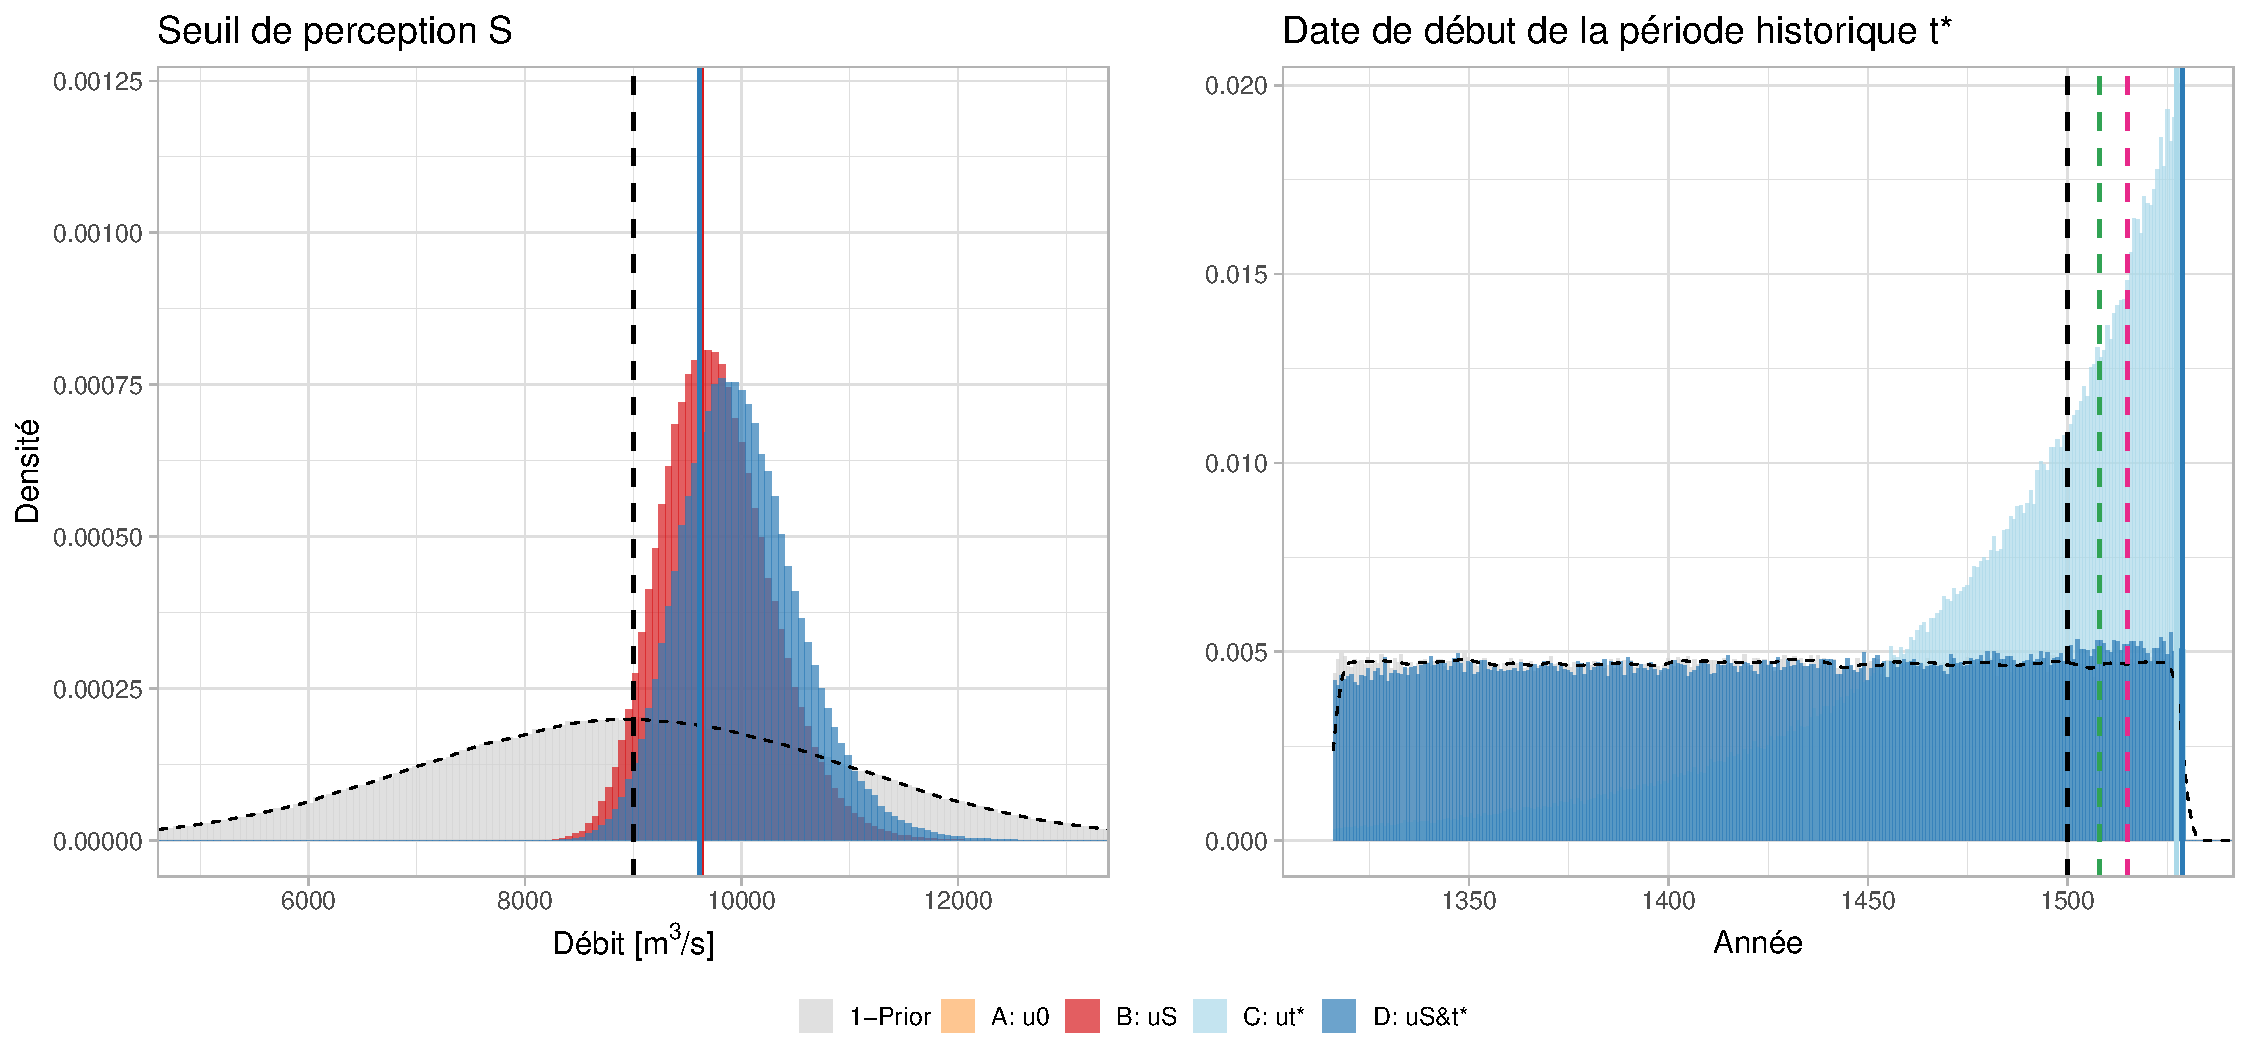
\includegraphics[width=.9\linewidth]{Figures/Params_C4.pdf}	
		\caption{Distributions a priori et a posteriori pour le seuil de perception (gauche) et la date de début de la période historique (droite). Les droites verticales pleines représentent l'estimation maxpost du paramètre pour chacun des modèles et les droites en pointillés noirs représentent les valeurs de référence. Les droites verticales en pointillés vert et rose représentent respectivement les estimations de $t*$ par la méthode de \cite{prosdocimi_german_2018} et par la méthode de la période de retour du seuil $S$.}
		\label{fig:Params_C4}
	\end{figure}

		\subsubsection{Quel est l'apport des crues historiques pour l'analyse fréquentielle à Beaucaire ?}

	 De la même manière qu'avec l'échantillon dégradé, on observe ici que la méconnaissance du seuil de perception (B et D) a plus d'impact sur l'incertitude des résultats que la méconnaissance de la durée de la période historique (C et D). De plus, l'incertitude autour des résultats est plus faible que celle de la référence uniquement dans les cas où le seuil de perception est supposé connu (modèles A et C). L'utilisation du nombre d'occurrences de crues historiques supérieures à un seuil ne permet de réduire l'incertitude autour des quantiles estimés que lorsque le seuil de perception est supposé parfaitement connu. L'utilisation d'a priori plus informatifs pourrait probablement donner des résultats moins incertains et plus réalistes quant à la connaissance du seuil de perception et de la durée de la période historique.
	 
	 \subsection{L'estimation des quantiles à Beaucaire (1500-2020) avec des a priori plus informatifs rend-elle l'utilisation des données historique plus pertinente ?}


	\paragraph{} Après analyse des résultats des modèles pour différents échantillons, il apparait que l'estimation la plus prudente des quantiles de crues à Beaucaire (1500-2020) consiste à utiliser le modèle D ($S$ et $n$ incertains) en parallèle d'une élicitation d'a priori relativement informatifs. L'utilisation de l'échantillon correspondant au seuil de perception le plus grand est également plus légitime. Il s'agit ici du seuil $S4$. 
	\paragraph{} La distribution a priori du seuil de perception $S4$ est à nouveau gaussienne et centrée sur la valeur supposée de 9000 m\textsuperscript{3}/s, en accord avec les estimations de \citet{pichard_hydro-climatology_2017} et des résultats du chapitre 2 (REF). L'écart type de la distribution est fixé à 500 m\textsuperscript{3}/s, ce qui le rend l'a priori plus informatif que lors des calculs précédents. En ce qui concerne la date de début de la période historique $t*$, une distribution est conservée pour l'a priori. La borne supérieure de la distribution reste fixée à la date de la première crue de la série (en 1529). En revanche, la borne inférieure est affectée à deux fois la durée que sépare la date de la première crue (1529) et la valeur supposée de $t*$ (1500), soit 58 ans. La borne inférieure de la distribution a priori est donc l'année 1471. La valeur théorique calculée en utilisant la méthode proposée par \citet{prosdocimi_german_2018} est 1510, elle est bien comprise dans la distribution a priori. Il en est de même pour la valeur théorique de $t*$ correspondant à la différence entre la période de retour du seuil de perception $S4$ (environ 15 ans) et la date de la première crue, ce qui correspond à l'année 1515.

	\begin{figure}[h]
		\centering
		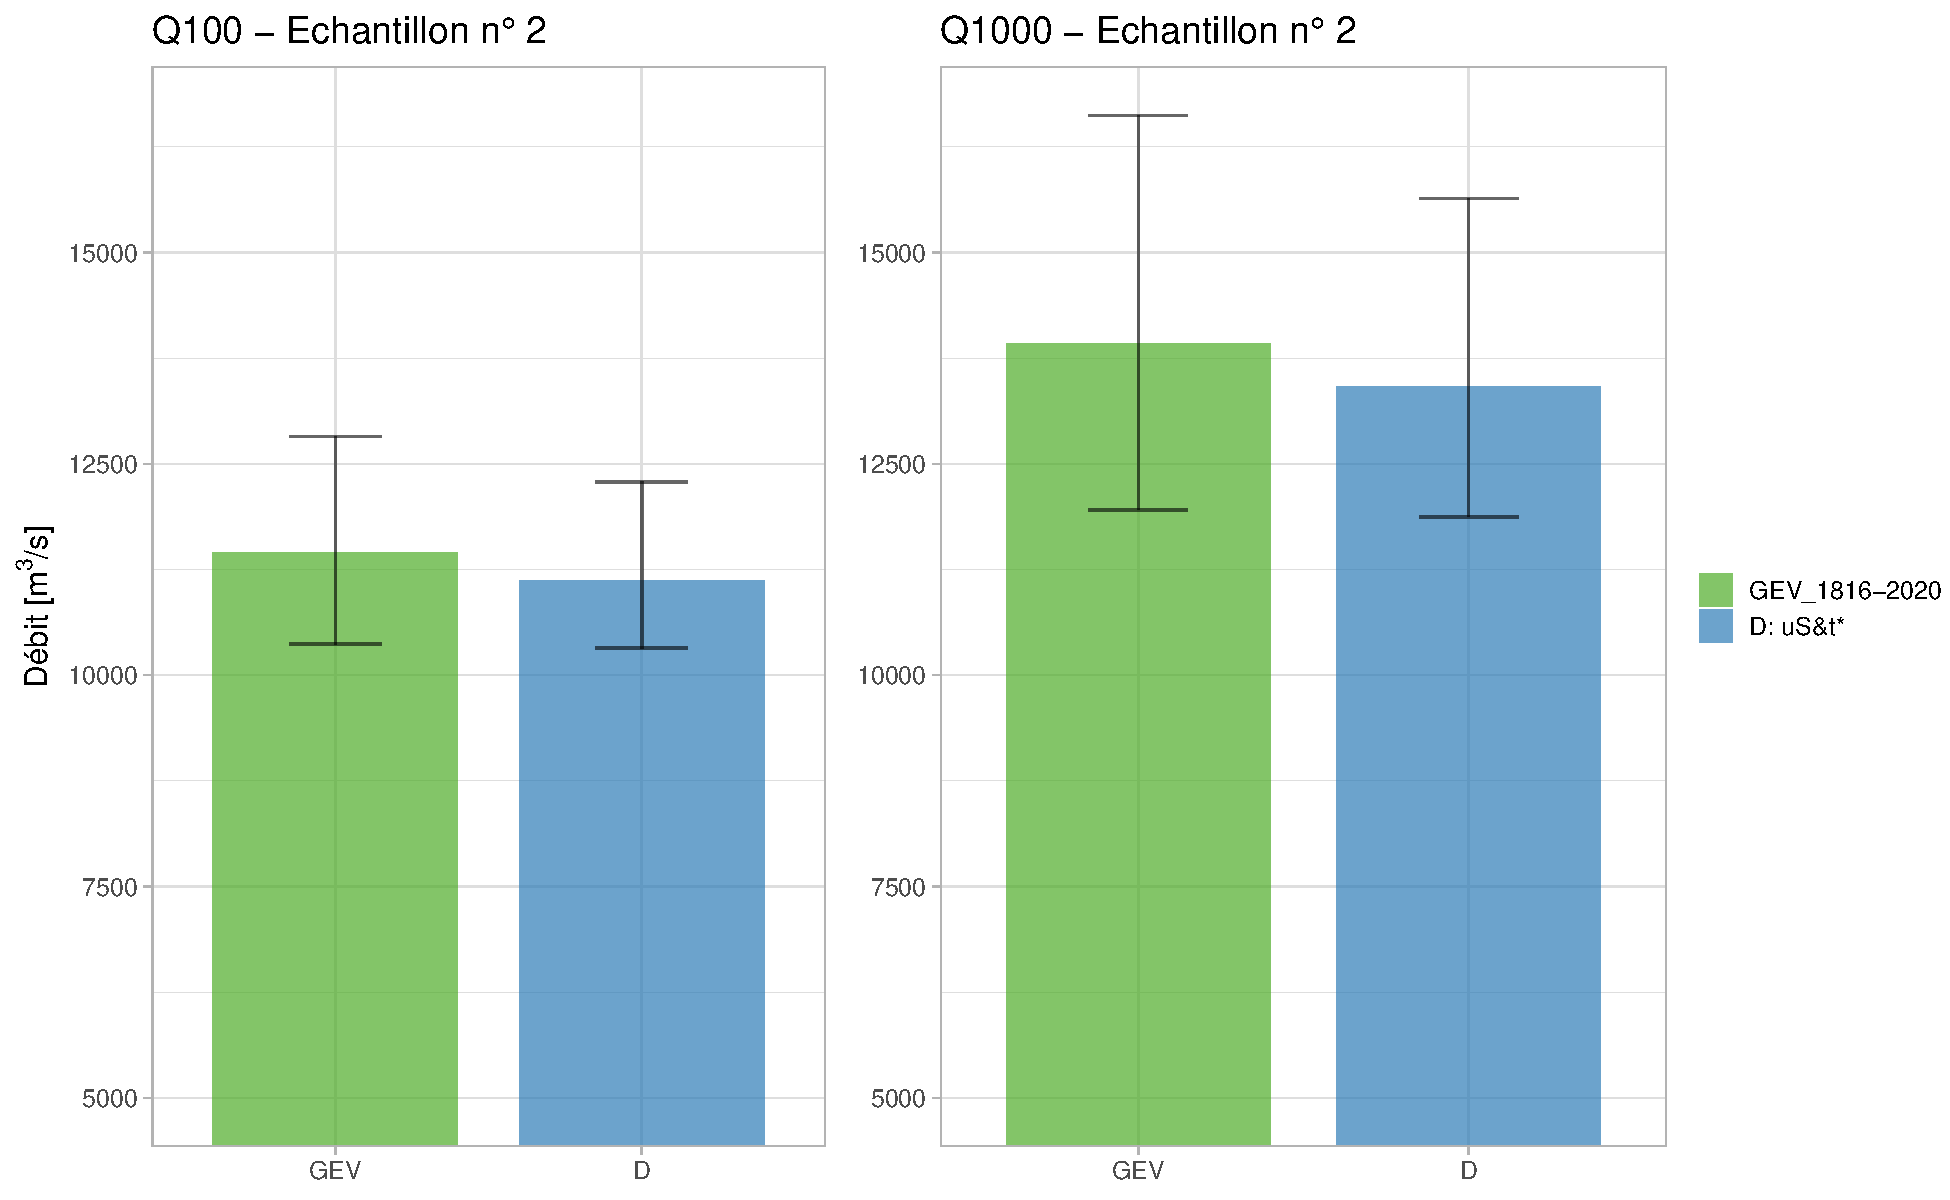
\includegraphics[width=.8\linewidth]{Figures/Barplots_QX_C4short.pdf}
		\caption{Estimations maxpost et incertitudes à 95\% pour Q100 et Q1000 par 2 modèles différents pour l'échantillon 2 (1500-2020, $S4$) après révision des distributions a priori de $S4$ et $n$.}
		\label{fig:BarplotC4short}
	\end{figure}

	\paragraph{} Les résultats du modèle D avec ces nouveaux a priori sont présentés dans la figure \ref{fig:BarplotC4short} ainsi que le tableau \ref{tab:ResC4short} et comparés avec les estimations GEV 1816-2020. Les quantiles du modèle D sont moins incertains que ceux de la référence. L'utilisation des crues historiques apparait pertinente pour réduire l'incertitude des quantiles, même dans le cas où $S$ et $n$ sont incertains. L'utilisation d'a priori plus informatifs a permis de réduire d'environ 25\% l'écart type de la distribution a posteriori de la crue millénale par rapport à des a priori très peu informatifs. 

	\begin{table}[h]
	\centering
	\resizebox{\columnwidth}{!}{%
		\begin{tabular}{|c|c|c|c|c|c|c|c|c|c|c|}
		\hline
Modèle & Q100 [m\textsuperscript{3}/s] & uQ100 [m\textsuperscript{3}/s] & Q1000 [m\textsuperscript{3}/s] & uQ1000 [m\textsuperscript{3}/s] & $\xi$ & $u\xi$ & $S$ [m\textsuperscript{3}/s] & $uS$ [m\textsuperscript{3}/s] & $t*$ & $ut*$ \\ \hline
GEV 1816-2020 & 11451 & 687   & 13919 & 1351   & 0.058 & 0.044  & X    & X    & X    & X \\ \hline
D             & 11118 & 585   & 13421 & 1110   & 0.063 & 0.040  & 9386 & 334  & 1526 & 17 \\ \hline
		\end{tabular}}
		\caption{Résultats maxpost et incertitudes de 2 modèles pour l'échantillon 2 après révision des distributions a priori de $S4$ et $n$. Q100 et Q1000 représentent respectivement le débit des crues centennales et millénales, $\xi$ le paramètre de forme de la distribution GEV, $S$ le seuil de perception et $t*$ la date de début de la période historique. Les écarts type des distributions a posteriori sont représentés par les colonnes débutant par la lettre "u".}
		\label{tab:ResC4short}
	\end{table}
		
	\paragraph{} Les distributions a posteriori de $S$ et $t*$ sont présentées dans la figure \ref{fig:Params_C4short}. Une fois de plus, la distribution a posteriori du seuil de perception est décalée vers des valeurs plus élevées que la valeur supposée de 9000 m\textsuperscript{3}/s, avec un seuil maxpost à 9386 m\textsuperscript{3}/s. La distribution a posteriori de $t*$ est à nouveau très proche de la distribution a priori, avec une densité un peu plus élevée pour les années proches de la date de la première crue. L'estimation maxpost de $t*$ est ici 1526, soit une durée de la période historique $n$ 26 ans plus courte qu'attendu. Cette sous-estimation de $n$ est non-seulement due au fait que les valeurs théoriques de la durée de la période historique sont plus petites que la durée supposée mais aussi à la probable non-exhaustivité des données historiques décrite dans la section précédente.	
			
	\begin{figure}[h]
		\centering
		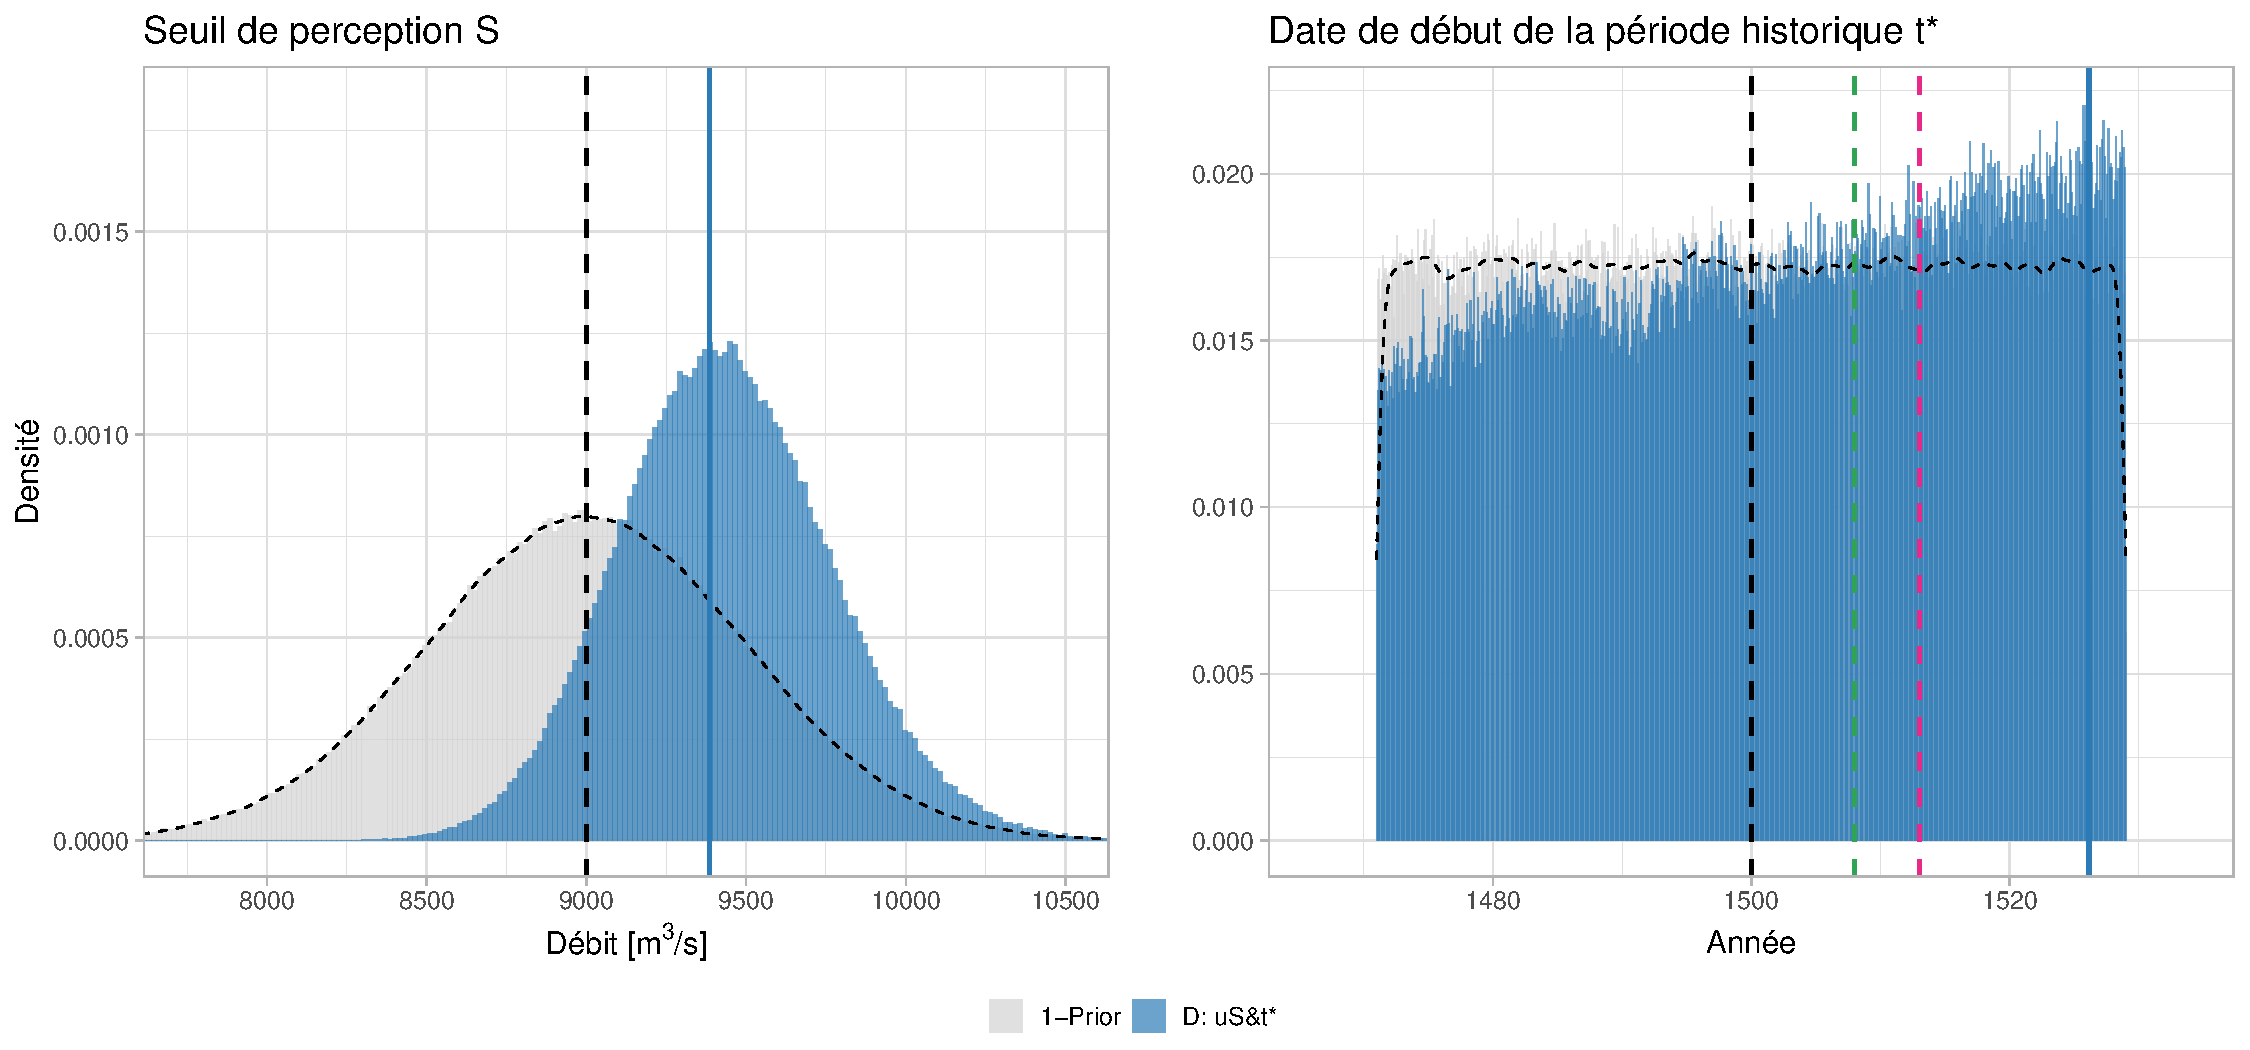
\includegraphics[width=.9\linewidth]{Figures/Params_C4short.pdf}	
		\caption{Distributions a priori et a posteriori pour le seuil de perception (gauche) et la date de début de la période historique (droite). Les droites verticales représentent l'estimation maxpost du paramètre de forme pour chacun des modèles. La droite verticale noire représente la date de début supposée de la chronique historique, ici 1500.}
		\label{fig:Params_C4short}
	\end{figure}
	
	\FloatBarrier
	
	\section{Discussion}
	
	\paragraph{} L'intérêt de la valorisation des données historiques pour l'analyse fréquentielle des crues est connu et étudié depuis longtemps (REF Stedinger, Autres). L'utilisation de données anciennes doit être accompagnée d'une estimation complète des incertitudes. Lors de l'utilisation d'un échantillon d'occurrences de crues supérieures à un seuil (le débit des crues historiques supérieures au seuil de perception n'est pas connu), la méconnaissance du seuil de perception et de la durée de la période historique est souvent négligée. Seule l'incertitude provenant de l'estimation des paramètres de la distribution choisie est généralement considérée. Quatre modèles sont proposés dans ce chapitre permettant de prendre en compte la méconnaissance autour de ces deux paramètres. La propagation de l'incertitude des débits de la période récente est également effectuée. 
	
	\paragraph{} Les modèles ont dans un premier temps été testés avec des a priori très peu informatifs et sur un échantillon continu artificiellement dégradé afin de se replacer dans un contexte historique. Ainsi, seuil de perception et durée de la période historique sont parfaitement connus. Les quantiles estimés ont été comparés avec les estimations d'un modèle GEV pour l'entièreté de la période (figure \ref{fig:Barplot_Artif2}). Il est apparu que considérer le seuil de perception comme étant incertain avait bien plus d'impact sur l'incertitude des résultats que considérer une méconnaissance sur la durée de la période historique. En revanche, quand ces deux paramètres sont considérés incertains en même temps, l'incertitude autour des quantiles est réduite par rapport au cas où seul le seuil est incertain. Une corrélation entre les distributions a posteriori de ces deux paramètres a été mise en évidence. Cette corrélation n'est pas surprenante étant donné que seuil et durée de la période historique sont par définition reliés : le nombre de dépassements du seuil de perception $k$ est à la fois dépendant du seuil $S$ et de la durée $n$. L'élicitation d'a priori plus informatifs pour ces deux paramètres est donc nécessaire. Bien que le seuil de perception soit un objet parfois difficile à cerner, il est donc possible de représenter sa méconnaissance à l'intérieur même du modèle fréquentiel. Considérer que le seuil de perception est parfaitement connu lorsque ce n'est pas le cas peut mener à une importante sous-estimation de l'incertitude des quantiles, de même que pour la durée de la période historique, dans une moindre mesure.
	
	\paragraph{} L'estimation du modèle binomial pour $S$ et $n$ connus (modèle A) a ensuite été comparée à une estimation pour laquelle le débit des crues historiques est connu et situé dans un intervalle (modèle E) pour l'échantillon dégradé. L'incertitude des résultats du modèle E se situe entre celle du modèle A et celle du modèle GEV pour l'ensemble de la période. Dans ce cas précis, l'utilisation du débit des crues historiques s'est donc avérée légèrement plus informative que l'utilisation du seul nombre de dépassements du seuil de perception. D'après \citet{payrastre_usefulness_2011}, la magnitude du seuil de perception utilisé influe directement sur l'incertitude des résultats dans le cas du modèle binomial. Ainsi, pour un seuil de perception suffisamment grand, l'incertitude des estimations du modèle binomial est identique à celle du modèle pour lequel le débit des crues historique est connu. L'intérêt de connaitre précisément le débit des crues historique est dans ce cas moins légitime. \citet{payrastre_usefulness_2011} estime que l'on se trouve dans cette situation lorsque la période de retour du seuil de perception est supérieur à environ 50 ans (dans les cas testés). A Beaucaire, la période de retour du seuil de perception $S4$ est d'environ 15 ans. Le seuil de perception est donc trop faible pour se trouver dans le cas où la connaissance des débits historiques n'est pas plus informative que la connaissance du nombre de dépassements du seuil. MICHEL : "Formulation plus "positive" : On dispose donc d'un recensement suffisant de crues historiques pour qu'il soit intéressant d'exploiter la connaissance du débit de ces crues, plutôt que de simplement comptabiliser le nombre de dépassements du seuil de perception".
	
		\paragraph{} Dans le cas l'échantillon de crues de Beaucaire de 1500 à 2020, l'utilisation des données anciennes reste, en l'absence d'estimations du débit des crues historiques, conditionnée à l'utilisation des seuils de perception de la base HISTRHÔNE : $S3$ ou $S4$. L'estimation des quantiles étant plus précise pour un seuil de perception correspondant à une période de retour importante, il est naturel de préférer le seuil $S4$. Il parait également plus prudent d'utiliser le modèle qui fait l'hypothèse d'une méconnaissance du seuil de perception et de la durée de la période historique (modèle D), en parallèle d'une élicitation réaliste des a priori de ces deux paramètres. Les résultats du modèle D sous les conditions décrites précédemment sont légèrement plus informatifs que l'utilisation de la seule chronique continue de 1816 à 2020 (figure \ref{fig:BarplotC4short}). Cela permet donc de conclure sur l'intérêt de l'utilisation des données historiques dans le cas de Beaucaire. Néanmoins, des doutes subsistent sur l'exhaustivité de l'échantillon historique. 
	
	\paragraph{} L'application des quatre modèles à l'échantillon complet de 1500 à 2020 à Beaucaire avec des a priori peu informatifs a montré que les estimations de la durée historique et du seuil de perception étaient différentes des valeurs supposées. Les modèles B et D estiment un seuil de perception plus grand que supposé et les modèles C et D estiment une durée de la période historique légèrement plus courte que celle supposée (figure \ref{fig:Params_C4}). Cette tendance pourrait être le symptôme d'une non-exhaustivité des crues dans les échantillons historiques de la base HISTRHÔNE, et ce bien qu'aucune non-homogénéité de la fréquence des crues n'ait été détectée (SECTION REF). Le nombre $k$ de dépassements du seuil de perception est donc possiblement sous-estimé dans les données disponibles. Cette sous-estimation pourrait provenir de la nature même des données, qui ne sont pas des données de crues supérieures à un seuil à part entière. Les catégories de la base HISTRHÔNE sont définies sur la perception des dommages par les populations ripariennes et non un seuil de perception physique directement lié au dépassement d'un débit. Or, comme décrit au chapitre 2 (REF), la perception des dommages par les populations a probablement évolué au cours du temps. JÉRÔME : "la "perception" n'est pas seulement déterminée par le débit (max) ou la hauteur d'eau (max) mais par plein d'autres facteurs physiques et humains : facteurs entraînant les dommages (qui déterminent plus directement la perception que le débit), eg durée, rupture de digue, saison, embâcles (dont glace!!), vulnérabilité / occupation du lit majeur,densité de population, contexte politique, médiatique (genre moine spécialisé dans le secteur, sachant écrire), conservation des archives, etc."
	
	\paragraph{} Suite à ce constat, on pourrait penser à l'utilisation d'un modèle qui considère non-seulement $S$ et $n$ comme étant incertains, mais également pour lequel le nombre de dépassements $k$ du seuil de perception est lui aussi incertain. Néanmoins, la méconnaissance du seuil de perception est déjà considérée comme étant particulièrement impactante sur les résultats. Lorsqu'il existe un tel doute sur l'exhaustivité des données historiques, discuter de l'incertitude du seuil de perception ou de la durée de la période historique parait secondaire. Ici, l'utilisation même des données historique pourrait être remise en cause. A DEVELOPPER
	
	\paragraph{} Il est probable que les données utilisées ici soient impactées par une variabilité climatique et/ou anthropique qui pourrait fragiliser l'hypothèse de stationnarité nécessaire à l'analyse fréquentielle, bien que l'homogénéité des données ait été vérifiée. Néanmoins, la non-prise en compte de ces sources de variabilité a probablement moins d'impact que la méconnaissance autour des données historiques. A DEVELOPPER OU DEPLACER EN CONCLUSION/PERSPECTIVES	

	
\section{Conclusion du chapitre}
	Conclusions sur l'intérêt des crues historiques pour l'estimation des quantiles extrêmes à Beaucaire. \\
	Est-ce qu'on observe une réelle amélioration par rapport aux résultats du chapitre 1 ?\\
	Selon les résultats, ajouter quelque chose comme : "l'utilisation des crues historiques peut mener à faire de fortes hypothèses (seuil et durée de la période), il faut être pragmatique sur la considération des incertitudes, même si elles mènent à des estimations incertaines des quantiles\\
	Ces conclusions sont valables uniquement à Beaucaire (période continue très longue, paramètre de forme positif, pas de tendance observée due au changement climatique ou autre). Mais que nous a appris l'application du modèle à un échantillon dégradé plus représentatif des longueurs de chronique habituelles ?\\
	Des a priori plus informatifs peuvent être élicités (comment ? Courbe de tarage Beaucaire / Arles, modélisation hydraulique ,...) \\
	Perspectives sur les modèles d'analyse fréquentielle en contexte non-stationnaire et sur les modèles régionaux.  

\printbibliography[title=Bibliographie]
\end{document}
